\chapter{Семейство внешних языков ostis-систем, близких языку внутреннего смыслового представления знаний}
\chapauthortoc{Садовский М.~Е.\\Голенков В.~В.\\Жмырко А.~В.\\Ефимова А.~А.}
\label{chapter_ext_lang}

\vspace{-7\baselineskip}
\begin{SCn}
\begin{scnrelfromlist}{автор}
	\scnitem{Садовский М.~Е.}
	\scnitem{Голенков В.~В.}
	\scnitem{Жмырко А.~В.}
	\scnitem{Ефимова А.~А.}
\end{scnrelfromlist}

\bigskip

\scntext{аннотация}{В главе рассматриваются понятия внешних и внутренних языков \textit{интеллектуальных компьютерных систем нового поколения}. Описываются внешние языки представления знаний в рамках \textit{Технологии OSTIS}, а именно \textit{SCg-код}, \textit{SCs-код} и \textit{SCn-код}. Для каждого из внешних языков детально рассматривается его \textit{синтаксис} и \textit{денотационная семантика}.}

\bigskip

\begin{scnrelfromlist}{подраздел}
	\scnitem{\ref{sec_identifiers}~\nameref{sec_identifiers}}
	\scnitem{\ref{sec_scg}~\nameref{sec_scg}}
	\scnitem{\ref{sec_scs}~\nameref{sec_scs}}
	\scnitem{\ref{sec_scn}~\nameref{sec_scn}}
\end{scnrelfromlist}

\bigskip

\begin{scnrelfromlist}{ключевое понятие}
	\scnitem{sc-идентификатор}
	\scnitem{SCg-код}
	\scnitem{SCs-код}
	\scnitem{SCn-код}
\end{scnrelfromlist}

\begin{scnrelfromlist}{ключевое знание}
	\scnitem{Правила построения sc-идентификаторов}
	\scnitem{Синтаксис и Денотационная семантика SCg-кода}
	\scnitem{Синтаксис и Денотационная семантика SCs-кода}
	\scnitem{Синтаксис и Денотационная семантика SCn-кода}
\end{scnrelfromlist}

\bigskip

\begin{scnrelfromlist}{библиография}
	\scnitem{\scncite{Standart2021}}
	\scnitem{\scncite{Golenkov2014b}}
	\scnitem{\scncite{IMS}}
	\scnitem{\scncite{Zhmyrko2022}}
	\scnitem{\scncite{Ostis-scn-latex-plugin2023}}
	\scnitem{\scncite{Ostis-standart2023}}
	\scnitem{\scncite{Ostis-tex2scs-translator2023}}
\end{scnrelfromlist}
\end{SCn}

\section*{Введение в Главу \ref{chapter_ext_lang}}

Для эксплуатации \textit{интеллектуальных компьютерных систем нового поколения} кроме способа абстрактного внутреннего представления \textit{баз знаний} требуются способы внешнего изображения абстрактных текстов, удобных для пользователей и используемых при оформлении исходных текстов \textit{баз знаний} указанных \textit{интеллектуальных компьютерных систем} и исходных текстов фрагментов этих \textit{баз знаний}, а также используемых для отображения пользователям различных фрагментов \textit{баз знаний} по пользовательским запросам(см. \scncite{Standart2021}).

В рамках данной главы рассматриваются правила идентификации \textit{sc-элементов}, а также \textit{внешние языки ostis-систем} (\textit{SCg-код}, \textit{SCs-код}, \textit{SCn-код}), которые являются различными вариантами внешнего представления текстов \textit{SC-кода}(см. Главу \ref{chapter_sc_code}~\nameref{chapter_sc_code}). Такие языки являются универсальными и, следовательно, семантически эквивалентными языками. Для каждого из указанных \textit{внешних языков} определяется его \textit{синтаксис} и \textit{денотационная семантика}.


\section{Внешние идентификаторы sc-элементов --- знаков, входящих в конструкции SC-кода}
\label{sec_identifiers}

\begin{SCn}
\begin{scnrelfromlist}{подраздел}
	\scnitem{\ref{sec_identifier_concept}~\nameref{sec_identifier_concept}}
	\scnitem{\ref{sec_main_and_system_identifiers_concept}~\nameref{sec_main_and_system_identifiers_concept}}
	\scnitem{\ref{sec_non_translation_identifier_concept}~\nameref{sec_non_translation_identifier_concept}}
	\scnitem{\ref{sec_simple_identifier_concept}~\nameref{sec_simple_identifier_concept}}
	\scnitem{\ref{sec_complex_identifier_concept}~\nameref{sec_complex_identifier_concept}}
\end{scnrelfromlist}	
	
\bigskip
	
\begin{scnrelfromlist}{ключевое понятие}
	\scnitem{sc-идентификатор}
	\scnitem{основной sc-идентификатор}
	\scnitem{неосновной sc-идентификатор}
	\scnitem{часто используемый sc-идентификатор}
	\scnitem{строковый sc-идентификатор}
	\scnitem{нестроковый sc-идентификатор}
	\scnitem{системный sc-идентификатор}
	\scnitem{нетранслируемый sc-идентификатор}
	\scnitem{локальный нетранслируемый sc-идентификатор}
	\scnitem{глобальный нетранслируемый sc-идентификатор}
	\scnitem{простой sc-идентификатор}
	\scnitem{sc-выражение}
	\scnitem{имя собственное}
	\scnitem{имя нарицательное}
\end{scnrelfromlist}

\begin{scnrelfromlist}{ключевое знание}
	\scnitem{Правила построения sc-идентификаторов}
	\scnitem{Правила построения основных sc-идентификаторов}
	\scnitem{Правила построения системных sc-идентификаторов}
	\scnitem{Правила построения нетранслируемых sc-идентификаторов}
	\scnitem{Правила построения простых sc-идентификаторов}
	\scnitem{Правила построения сложных sc-идентификаторов}
\end{scnrelfromlist}
\end{SCn}

\subsection{Понятие sc-идентификатора sc-элемента}
\label{sec_identifier_concept}

\scnkeyword{sc-идентификатор} (или \textit{внешний идентификатор sc-элемента}) необходим \mbox{\textit{ostis-системе}} исключительно для того, чтобы осуществлять обмен информацией с другими \textit{ostis-системами} или со своими пользователями. Для того чтобы представить свою \textit{базу знаний}, решать самые различные \textit{задачи}, связанные с анализом текущего состояния и эволюцией своей \textit{базы знаний}, задачи, связанные с анализом текущего состояния (текущих ситуаций) окружающей среды, принятием соответствующих решений (целей) и организацией соответствующих \textit{действий}, направленных на выполнение принятых решений (на достижение поставленных целей), \textit{ostis-системе} не нужны никакие внешние идентификаторы (в частности, имена) соответствующие \textit{sc-элементам}. Но для понимания сообщений, принимаемых от других субъектов (что для \textit{ostis-системы} означает построение \textit{sc-текста},~~ \textit{семантически эквивалентного} принятому сообщению) и для анализа сообщений, передаваемых другим субъектам (что для \textit{ostis-системы} означает синтез \textit{внешнего текста},~~\textit{семантически эквивалентного} заданному \textit{sc-тексту} и удовлетворяющего некоторым дополнительным требованиям, например, эмоционального характера) \textit{ostis-системе} необходимо знать, как в принимаемом или передаваемом сообщении изображаются (представляются) \textit{знаки}, синонимичные sc-элементам, которые уже хранятся или могут храниться в составе \textit{базы знаний}~~\textit{ostis-системы}. В качестве \textit{внешнего идентификатора sc-элемента} чаще всего используются имена (термины) соответствующих (обозначаемых) сущностей, представленные отдельными словами или словосочетаниями на различных естественных языках, но также могут использоваться иероглифы, условные обозначения, пиктограммы.

В общем случае \textit{sc-элементу} может соответствовать несколько синонимичных ему имен на разных \textit{естественных языках}. Более того, \textit{sc-элементу} может соответствовать несколько синонимичных ему имен на одном и том же \textit{естественном языке}. В этом случае одно из этих имен объявляется как \textit{основной внешний идентификатор} для соответствующего \textit{sc-элемента} и соответствующего \textit{естественного языка}. Основное требование, предъявляемое к таким внешним идентификаторам это отсутствие как синонимов, так и омонимов в рамках множества \textit{основных внешних идентификаторов sc-элементов} для каждого естественного языка. 

Каждый \textit{внешний идентификатор sc-элемента}, используемый \textit{ostis-системой}, может быть описан (представлен) в ее памяти в виде \textit{внутреннего файла ostis-системы}, то есть в виде электронного образа всевозможных вхождений данного внешнего идентификатора во всевозможные внешние тексты соответствующего внешнего языка. В некоторых случаях явное представление в памяти не требуется, например, в случае \textit{нетранслируемых sc-идентификаторов}.

Каждому sc-элементу может соответствовать целое семейство внешних идентификаторов этого \textit{sc-элемента}, которые обычно являются терминами, именующими обозначаемую сущность. Среди этих внешних идентификаторов для каждого идентифицируемого \textit{sc-элемента} выделяется один как основной идентификатор.
А неосновные термины (имена), соответствующие этим sc-элементам (в том числе и классам), поясняют \textit{денотационную семантику} указанного \textit{sc-элемента}.

\begin{SCn}
	\scnheader{sc-идентификатор}
	\scntext{часто используемый sc-идентификатор}{внешний идентификатор sc-элемента}
	\scnidtf{строка символов или пиктограмма, взаимно однозначно представляющая соответствующий sc-элемент, хранимый в sc-памяти}
	\begin{scnrelfromset}{разбиение}
		\scnitem{простой sc-идентификатор}
		\begin{scnindent}
			\scnidtf{простой внешний идентификатор sc-элемента}	
		\end{scnindent}
		\scnitem{sc-выражение}	
		\begin{scnindent}
			\scnidtf{сложный внешний идентификатор sc-элемента, в состав которого входит один или несколько идентификаторов других sc-элементов}	
		\end{scnindent}
	\end{scnrelfromset}
	\begin{scnrelfromset}{разбиение}
		\scnitem{основной sc-идентификатор}
		\begin{scnindent}
			\scnidtf{основной sc-идентификатор для носителей дополнительно указываемого языка общения (например, соответствующего естественного языка)}
			\scntext{примечание}{\textit{основной sc-идентификатор} является уникальным (не имеет синонимов и омонимов) в рамках соответствующего естественного языка}
			\scnsuperset{основной международный sc-идентификатор}	
		\end{scnindent}
		\scnitem{неосновной sc-идентификатор}	
		\begin{scnindent}	
			\scnsuperset{{\normalfont(}неосновной sc-идентификатор $\cap$ пояснение{\normalfont)}}
			\begin{scnindent}
				\scnidtf{неосновной sc-идентификатор, являющийся одновременно и пояснением обозначаемой сущности(см. \textit{\ref{sec_kb}~\nameref{sec_kb}})}
				\scnsuperset{{\normalfont(}неосновной sc-идентификатор $\cap$ определение{\normalfont)}}
				\begin{scnindent}
					\scnidtf{неосновной sc-идентификатор, являющийся одновременно и определением обозначаемого понятия(см. \textit{\ref{sec_kb}~\nameref{sec_kb}})}
				\end{scnindent}
			\end{scnindent}
			\scnsuperset{часто используемый sc-идентификатор}
		\end{scnindent}
	\end{scnrelfromset}
\end{SCn}

\subsection{Понятие основного и системного sc-идентификаторов sc-элемента}
\label{sec_main_and_system_identifiers_concept}

В качестве \textbf{\textit{основного sc-идентификатора}} могут использоваться также общепринятые международные условные обозначения некоторых сущностей, например, обозначения часто используемых функций (sin, cos, tg, log, и так далее), единиц измерения, денежных единиц и многое другое. Формально каждый \textit{основной международный sc-идентификатор} считается \textit{основным sc-идентификатором} также и для каждого \textit{естественного языка}, несмотря на то, что символы, используемые в \textit{основных международных sc-идентификаторах}, могут не соответствовать алфавиту некоторых или даже всех \textit{естественных языков}.

С помощью \textit{неосновного sc-идентификатора} указываются возможные \textit{синонимы*} соответствующего \textit{основного sc-идентификатора}, которые в частности, могут пояснять или даже определять обозначаемую сущность, указывает на важные свойства этой сущности.

Для некоторых \textit{sc-элементов} могут часто использоваться не только основной, но и \textit{неосновной sc-идентификатор} (особенно в неформальных текстах --- в пояснениях, примечаниях и тому подобных). Явное выделение такого класса \textit{sc-идентификаторов} позволяет упростить семантический анализ исходных текстов \textit{баз знаний}.

\textbf{\textit{системный sc-идентификатор}} --- это \textit{sc-идентификатор}, являющийся уникальным в рамках всей базы знаний \textit{Экосистемы OSTIS}. Данный \textit{sc-идентификатор}, как правило, используется в исходных текстах \textit{базы знаний}, при обмене сообщениями между \textit{ostis-системами}, а также для взаимодействия \textit{ostis-системы} с компонентами, реализованными с использованием средств, внешних с точки зрения \textit{Технологии OSTIS}, например, программ, написанных на традиционных языках программирования. Алфавит \textit{системных sc-идентификаторов} максимально упрощен для того, чтобы обеспечить удобство автоматической обработки таких \textit{sc-идентификаторов} с использованием современных технических средств, в частности, запрещены пробелы и различные специальные символы.

\begin{SCn}
	\scnheader{основной sc-идентификатор}
	\scnsubset{файл-образец ostis-системы}
	\scnrelboth{семантическая эквивалентность}{\scnfilelong{Все \textit{основные идентификаторы sc-элементов} в памяти \textit{ostis-системы} оформляются в виде копируемых файлов-образцов ostis-системы. Аналогичное утверждение справедливо и для неосновных \textit{часто используемых sc-идентификаторов}. Все остальные \textit{неосновные sc-идентификаторы} считаются вспомогательными файлами-экземплярами.}}
	\begin{scnindent}
		\scntext{пояснение}{Копии основных sc-идентификаторов входят в состав внешних текстов различных языков (\textit{SCg-кода}, \textit{SCs-кода}, \textit{SCn-кода}), а также в различных падежах, склонениях, спряжениях в состав \textit{файлов ostis-систем}.}
	\end{scnindent}

	\scnheader{sc-идентификатор}
	\begin{scnrelfromset}{разбиение}
		\scnitem{строковый sc-идентификатор}
		\begin{scnindent}
			\scnidtf{sc-идентификатор, представленный строкой символов, которая является именем обозначаемой сущности}
			\scnidtf{имя сущности, обозначаемой идентифицируемым sc-элементом}
			\scnidtf{имя (термин, словосочетание), синонимичное соответствующему (идентифицируемому) \mbox{sc-элементу} и представленное в соответствующем алфавите символов}
		\end{scnindent}
		\scnitem{нестроковый sc-идентификатор}	
		\begin{scnindent}
			\scntext{пояснение}{В общем случае в качестве \textit{sc-идентификатора} некоторого \textit{sc-элемента} может выступать произвольный \textit{внутренний файл ostis-системы}, например, пиктограмма, условное обозначение или даже аудиофрагмент.}	
		\end{scnindent}
	\end{scnrelfromset}
	\scntext{примечание}{Введенные нами \textit{sc-идентификаторы} используются во всех \textit{внешних языках}, близких \textit{SC-коду} --- в \textit{SCg-коде}, \textit{SCs-коде} и \textit{SCn-коде}.}
	
	\scnheader{строковый sc-идентификатор}
	\scnidtf{имя, приписываемое идентифицируемому sc-элементу}
	\scnidtf{имя сущности, обозначаемой идентифицируемым sc-элементом}
	\scnidtf{строка символов, синонимичная соответствующему идентифицируемому sc-элементу}
	\scnsuperset{основной строковый sc-идентификатор}
	\begin{scnindent}
		\scnidtf{уникальное для каждого естественного языка внешнее имя, приписываемое идентифицируемому sc-элементу}
		\scnsuperset{основной русскоязычный sc-идентификатор}
		\scnsuperset{системный sc-идентификатор}
		\scnsuperset{основной англоязычный sc-идентификатор}
		\scnsuperset{основной германоязычный sc-идентификатор}
		\scnsuperset{основной франкоязычный sc-идентификатор}
		\scnsuperset{основной италоязычный sc-идентификатор}
		\scnsuperset{основной китайскоязычный sc-идентификатор}
	\end{scnindent}
	\scnsuperset{системный sc-идентификатор}
\end{SCn}

Символами, использующимися в \textit{системном sc-идентификаторе}, могут быть буквы латинского алфавита, цифры, знак нижнего подчеркивания и знак тире. Для обеспечения интернационализации рекомендуется формировать \textit{системные sc-идентификаторы} на основании основных англоязычных \textit{sc-идентификаторов}. Таким образом, наиболее целесообразно формировать \textit{системный sc-идентификатор} \textit{sc-элемента} из основного англоязычного путем замены всех символов, не входящих в описанный выше алфавит на символ нижнее подчеркивание (``\_''). Кроме того, заглавные буквы чаще всего заменяются на соответствующие строчные.

Для именования \textit{sc-элементов}, являющихся знаками \textit{ролевых отношений}, вместо знака \scnqqi{\scnrolesign} в \textit{системном sc-идентификаторе} используется приставка \scnqqi{rrel} и далее после нижнего подчеркивания записывается имя \textit{ролевого отношения}. Для именования sc-элементов, являющихся знаками \textit{неролевых отношений}, вместо знака \scnqqi{*} в \textit{системном sc-идентификаторе} используется приставка \scnqqi{nrel} и далее после нижнего подчеркивания записывается имя \textit{неролевого отношения}. Для именования sc-элементов, являющихся знаками классов \textit{понятий} в \textit{системном sc-идентификаторе} используется приставка \scnqqi{concept} и далее после нижнего подчеркивания записывается имя \textit{класса}. Для именования sc-элементов, являющихся знаками \textit{структур} в \textit{системном sc-идентификаторе} используется приставка \scnqqi{struct} и далее после нижнего подчеркивания записывается имя \textit{структуры}.

\subsection{Понятие нетранслируемого sc-идентификатора sc-элемента}
\label{sec_non_translation_identifier_concept}

\begin{SCn}
	\scnheader{нетранслируемый sc-идентификатор}
	\scnsubset{системный sc-идентификатор}
	\scnidtf{sc-идентификатор, не представляемый в базе знаний ostis-системы}
	\scnidtf{sc-идентификатор, существующий только вне базы знаний ostis-системы}
	\begin{scnrelfromset}{разбиение}
		\scnitem{глобальный нетранслируемый sc-идентификатор}
		\scnitem{локальный нетранслируемый sc-идентификатор}
	\end{scnrelfromset}
\end{SCn}

\textbf{\textit{нетранслируемый sc-идентификатор}} используется только в рамках исходных текстов \textit{баз знаний} (в том числе, \textit{sc.s-текстов}) и при обмене сообщениями между \textit{ostis-системами} в тех случаях, когда необходимо в нескольких фрагментах исходного текста \textit{базы знаний} или передаваемого сообщения использовать имя одного и того же \textit{sc-элемента}, но при этом указанный \textit{sc-элемент} не имеет \textit{системного sc-идентификатора} и вводить его нецелесообразно. Использование \textit{нетранслируемого sc-идентификатора} позволяет повысить читабельность и структурированность исходных текстов \textit{баз знаний}, а также позволяет обратиться к одному и тому же неименуемому (в рамках базы знаний) \textit{sc-элементу} в разных файлах исходных текстов \textit{баз знаний} или в разных сообщениях, передаваемых между \textit{ostis-системами}. В качестве таких \textit{sc-элементов} часто выступают знаки \textit{структур} и \textit{связок}.

Таким образом, \textit{нетранслируемый sc-идентификатор} существует только вне \textit{базы знаний ostis-системы} и при формировании \textit{базы знаний} из исходных текстов или при погружении в \textit{базу знаний} полученного сообщения соответствующий им \textit{внутренний файл ostis-системы} не создается.

\textit{нетранслируемый sc-идентификатор} строится по тем же принципам, что и \textit{системный sc-идентификатор}, но в начале \textit{нетранслируемого sc-идентификатора} ставится одна или несколько точек (\scnqqi{.}), количество которых определяет область видимости данного \textit{нетранслируемого sc-идентификатора}.

\textbf{\textit{глобальный нетранслируемый sc-идентификатор}} считается уникальным в рамках всего имеющегося набора исходных текстов \textit{баз знаний} и/или передаваемых между \textit{ostis-системами} сообщений. Таким образом, \textit{sc-элементы}, имеющие на уровне исходных текстов (в том числе, в разных файлах исходных текстов) одинаковый \textit{глобальный нетранслируемый sc-идентификатор}, считаются синонимичными и в \textit{базе знаний ostis-системы} представляются одним и тем же \textit{sc-элементом}.

Можно сказать, что областью видимости \textit{глобального нетранслируемого sc-идентификатора} является весь набор (репозиторий) исходных текстов некоторой \textit{базы знаний}. В начале \textit{глобального нетранслируемого sc-идентификатора} ставится одна точка.

\textbf{\textit{локальный нетранслируемый sc-идентификатор}} считается уникальным в рамках \myuline{конкретного} файла исходных текстов \textit{баз знаний} и/или передаваемого между \textit{ostis-системами} сообщения. Таким образом, \textit{sc-элементы}, имеющие в рамках одного файла исходных текстов одинаковый \textit{локальный нетранслируемый sc-идентификатор}, считаются \myuline{синонимичными}, в то время как \textit{sc-элементы}, имеющие в рамках \myuline{разных} файлов исходных текстов одинаковый \textit{локальный нетранслируемый sc-идентификатор} будут считаться \myuline{разными} \textit{sc-элементами}.

Можно сказать, что областью видимости \textit{локального нетранслируемого sc-идентификатора} является конкретный файл исходных текстов \textit{базы знаний}. В начале \textit{локального нетранслируемого sc-идентификатора} ставится две точки.

Уникальный \textit{нетранслируемый sc-идентификатор} используется для однократного обозначения конкретного неименуемого \textit{sc-элемента} в рамках исходных текстов \textit{баз знаний} и/или передаваемых между \textit{ostis-системами} сообщений.

Кроме того, уникальный \textit{нетранслируемый sc-идентификатор} может использоваться при визуализации \textit{баз знаний} в виде, например, \textit{sc.s-текстов} или \textit{sc.n-текстов}, в тех случаях, когда необходимо визуализировать \textit{sc-элемент}, не имеющий \textit{sc-идентификатор}.

Каждое вхождение уникального \textit{нетранслируемого sc-идентификатора} в исходный текст \textit{базы знаний} или передаваемое сообщение считается обозначением \myuline{разных} \textit{sc-элементов} (чаще всего, \textit{sc-узлов}).

\begin{SCn}
	\scnheader{sc-идентификатор*}
	\scnsuperset{основной sc-идентификатор*}
	\begin{scnindent}
		\scnidtf{\textit{бинарное ориентированное отношение}, каждая пара которого связывает \textit{sc-элемент} с внутренним файлом \textit{ostis-системы}, который содержит \textit{основной sc-идентификатор} указанного \textit{sc-элемента}.}
		\scntext{примечание}{отношение, связывающее \textit{sc-элементы} с файлами, содержащими их \textit{основные sc-идентификаторы}, само имеет свой \textit{основной sc-идентификатор}, который представляет собой строку символов, имеющую вид \scnqqi{основной sc-идентификатор*}. Заметим, что в состав первого домена отношения \textit{\scnqqi{основной sc-идентификатор*}} входит также и \textit{sc-узел}, обозначающий само это отношение.}
	\end{scnindent}
	\scnsuperset{системный sc-идентификатор*}
	\begin{scnindent}
		\scnidtf{\textit{бинарное ориентированное отношение}, каждая пара которого связывает \textit{sc-элемент} с внутренним файлом \textit{ostis-системы}, который содержит \textit{системный sc-идентификатор} указанного \textit{sc-элемента}.}
	\end{scnindent}
\end{SCn}

\textit{системные sc-идентификаторы} отличаются от \textit{основных}, во-первых, требованием к уникальности в рамках всей \textit{базы знаний} \textit{Экосистемы OSTIS} (а, значит, независимостью от внешнего языка), а во-вторых, более простым алфавитом, удобным для автоматической обработки.

\textit{cистемные sc-идентификаторы} и \textit{нетранслируемые sc-идентификаторы} выполняют схожие функции, связанные с именованием \textit{sc-элементов} на уровне исходных текстов \textit{баз знаний} или передаваемых между \textit{ostis-системами} сообщений.

Каждый \textit{системный sc-идентификатор} представляется в \textit{базе знаний} в виде \textit{внутреннего файла ostis-системы} и связан с соответствующим \textit{sc-элементом} парой отношения \textit{системный \mbox{sc-идентификатор*}}. \textit{нетранслируемые sc-идентификаторы} не представляются в рамках \textit{базы знаний}, не имеют соответствующих \textit{внутренних файлов ostis-системы} и на уровне \textit{базы знаний} никак не связаны с идентифицируемыми ими \textit{sc-элементами}.

\subsection{Понятие простого sc-идентификатора sc-элемента}
\label{sec_simple_identifier_concept}

\textbf{\textit{простой sc-идентификатор}} --- \textit{sc-идентификатор sc-элемента}, в состав которого идентификаторы других sc-элементов не входят и который не содержит \textit{транслируемую в SC-код} информацию об обозначаемой им сущности. 

\textbf{\textit{простой строковый sc-идентификатор}} --- \textit{простой sc-идентификатор}, представляющий собой строку (цепочку) символов, которая является именем (названием) той же сущности, что и идентифицируемый sc-элемент. \textit{простые строковые sc-идентификаторы} являются наиболее распространенным видом идентификаторов, приписываемых sc-элементам.

\begin{SCn}
	\scnheader{простой строковый sc-идентификатор}
	\scnsuperset{системный sc-идентификатор}
	\scnsuperset{простой строковый идентификатор sc-переменной}
	\begin{scnindent}
		\scnhaselementrole{пример}{\scnfilelong{\_var1}}
	\end{scnindent}
	\scnsuperset{простой строковый sc-идентификатор неролевого отношения}
	\begin{scnindent}
		\scnidtf{простой строковый идентификатор sc-узла, являющегося знаком неролевого отношения}
		\scnhaselementrole{пример}{\scnfilelong{включение множеств*}}
	\end{scnindent}
	\scnsuperset{простой строковый sc-идентификатор ролевого отношения}
	\begin{scnindent}
		\scnidtf{простой строковый идентификатор sc-узла, являющегося знаком ролевого отношения}
		\scnhaselementrole{пример}{\scnfilelong{слагаемое\scnrolesign}}
	\end{scnindent}
	\scnsuperset{простой строковый sc-идентификатор класса классов}
	\begin{scnindent}
		\scnidtf{простой строковый идентификатор sc-узла, являющегося знаком класса классов}
		\scnhaselementrole{пример}{\scnfilelong{длина\scnsupergroupsign}}
	\end{scnindent}
	\scnsuperset{sc-идентификатор внешнего файла ostis-системы}
	\begin{scnindent}
		\scnidtf{URL-идентификатор}
		\scnhaselementrole{пример}{\scnfilelong{\scnqqi{file:///home/user/image1.png}}}
		\begin{scnindent}
			\scntext{примечание}{Данный sc-идентификатор описывает абсолютный путь к файлу под названием \scnqqi{image1.png}}
		\end{scnindent}	
		\scnhaselementrole{пример}{\scnfilelong{\scnqqi{file://image1.png}}}
		\begin{scnindent}
			\scntext{примечание}{Данный sc-идентификатор описывает относительный путь к файлу под названием \scnqqi{image1.png}}
		\end{scnindent}	
		
		\scnhaselementrole{пример}{\scnfilelong{\scnqqi{https://conf.ostis.net/content/image1.png}}}
		\begin{scnindent}
			\scntext{примечание}{Данный sc-идентификатор описывает путь к файлу под названием \scnqqi{image1.png}, расположенному на удаленном сервере.}
		\end{scnindent}	
	\end{scnindent}
\end{SCn}

\textbf{\textit{sc-идентификатор внешнего файла ostis-системы}} предназначен для описания местоположения \textit{внешнего файла ostis-системы} и представляет собой строку символов, которая строится в соответствии со стандартом URL, а затем берется в двойные кавычки. Кавычки нужны для однозначности определения того, где начинается и заканчивается данный \textit{sc-идентификатор}, поскольку в общем случае в URL разрешены пробелы. Целесообразность этого обусловлена тем, что \textit{sc-идентификаторы} данного типа часто используются в файлах исходных текстов баз знаний ostis-систем.

\textit{sc-идентификатор внешнего файла ostis-системы} с точки зрения \textit{Технологии OSTIS} является \textit{простым строковым sc-идентификатором}, хотя и может содержать специальные символы, например \scnqqi{\%} или \scnqqi{/}. Это связано с тем, что указанный идентификатор не несет в себе семантически значимой информации о свойствах самого \textit{sc-элемента}, обозначаемого таким \textit{sc-идентификатором}, а только информацию о его расположении в текущем состоянии внешнего мира \textit{ostis-системы}.

\textbf{\textit{имя нарицательное}} --- \textit{имя}, которое либо не является обозначением какого-либо класса сущностей, либо является обозначением (именем) некоторого класса сущностей, но построенным без использования нарицательного имени этого класса, либо является именем некоторого класса сущностей, построенным с использованием нарицательного имени этого класса либо путем преобразования имени нарицательного во множественное число, либо путем дополнительного использования в начале формулируемого имени таких слов или словосочетаний, как \scnqqi{Знак класса}, \scnqqi{Класс}, \scnqqi{Знак множества}, \scnqqi{Множество}, \scnqqi{Знак множества всевозможных}, \scnqqi{Множество всевозможных}. \textbf{\textit{имя собственное}} всегда начинается с большой буквы.

\textit{имя нарицательное} --- \textit{имя} некоторого класса сущностей (а, точнее, имя класса sc-элементов, обозначающих сущности некоторого класса), которое, с одной стороны, является знаком всего указанного класса, а, с другой стороны, соответствует (может быть приписано) любому экземпляру этого класса. \textit{имя нарицательное} всегда начинается с маленькой буквы.

\textbf{Правила построения простого строкового sc-идентификатора} включают в себя:
\begin{textitemize}
	\item алфавит символов, используемых в \textit{простых строковых sc-идентификаторах};
	\item префиксы и суффиксы, используемые в \textit{простых строковых sc-идентификаторах};
	\item разделители и ограничители, используемые в \textit{простых строковых sc-идентификаторах};
	\item правила построения \textit{имен собственных} и \textit{имен нарицательных}, являющихся простыми строковыми sc-идентификаторами;
	\item правила построения \textit{простых строковых sc-идентификаторов}, определяемые различными классами идентифицируемых \textit{sc-элементов}.
\end{textitemize}

Общим правилом построения \textit{простого sc-идентификатора} является стремление максимально возможным образом использовать сложившуюся терминологию. Но при этом следует подчеркнуть, что необходимость исключения омонимии в \textit{sc-идентификаторах} требует строгого формального \myuline{уточнения} семантической интерпретации каждого используемого термина. Особо подчеркнем то, что в \textit{ostis-системах} процесс построения новых терминов (\textit{sc-идентификаторов}) и процесс совершенствования существующей терминологии по отношению к процессу эволюции \textit{баз знаний}, представленных в \textit{SC-коде}, с технической точки зрения абсолютно не зависят друг от друга. Кроме того, следует помнить, что \myuline{далеко не все} \textit{sc-элементы}, входящие в состав базы знаний \textit{ostis-системы}, должны иметь соответствующие им \textit{sc-идентификаторы} (быть идентифицированными). Существенно подчеркнуть то, что далеко не все sc-элементы должны иметь \textit{простые sc-идентификаторы} по той простой причине, что для многих sc-элементов в случае необходимости можно достаточно легко построить идентифицирующее их \textit{sc-выражение} (sc-выражение). Тем не менее, для целого ряда сущностей (например, для понятий, исторических событий и тому подобных) обойтись без простых sc-идентификаторов очень сложно. Очевидно, что идентифицированными (именованными) должны быть все используемые понятия, вводимые в соответствующих предметных областях и специфицируемые соответствующими онтологиями. Идентифицированными также должны быть обладающие особыми свойствами ключевые экземпляры (элементы) некоторых понятий, различные социально значимые объекты (персоны, населенные пункты, географические объекты, страны, организации, библиографические источники, исторические события и многое другое).

Первым символом каждого \textit{простого строкового sc-идентификатора}, идентифицирующего \textit{sc-переменную} (переменный \textit{sc-элемент}), является \textit{знак подчеркивания}. При этом, если после указанного знака подчеркивания указывается \textit{имя нарицательное} некоторого \textit{класса sc-элементов}, то рассматриваемый \textit{простой строковый sc-идентификатор} становится уже \textit{sc-выражением}, содержащим информацию о том, что \textit{областью возможных значений*} идентифицируемой \textit{sc-переменной} является указанный \textit{класс sc-элементов}.

Последним символом \textit{простого строкового sc-идентификатора}, идентифицирующего \textit{sc-узел}, обозначающий \textit{неролевое отношение}, заданное на множестве \textit{sc-элементов}, является надстрочная \textit{звездочка}.

Последним символом \textit{простого строкового sc-идентификатора}, идентифицирующего \textit{sc-узел}, обозначающий заданное на множестве sc-элементов \textit{ролевое отношение} (то есть \textit{отношение}, являющееся подмножеством \textit{отношения принадлежности}), является \textit{штрих} (прямой апостроф).

Последним символом \textit{простого строкового sc-идентификатора}, идентифицирующего \textit{sc-узел}, обозначающий понятие, являющееся классом классов (таковыми в частности, являются различного рода параметры --- длина, площадь, объем, масса) является символ \textit{циркумфлекс} (\scnqqi{крышка}). Однако, если отсутствует омонимичный идентификатор без этого суффикса, то указанный символ можно не приписывать.

\textit{простой строковый sc-идентификатор} может рассматриваться как последовательное сокращение \textit{sc-идентификаторов} одного и того же \textit{sc-элемента} с преобразованием \textit{имен собственных} в \textit{имена нарицательные} и наоборот.

При наличии синонимичных \textit{имен собственных} и \textit{имен нарицательных} при выборе \textit{основного sc-идентификатора} преимущество имеют \textit{имена нарицательные}. Так, например, основным идентификатором \textit{sc-узла}, обозначающего \textit{SC-код}, является термин \scnqqi{\textit{sc-текст}}, а термин \scnqqi{\textit{SC-код}}, являющийся \textit{именем собственным}, считается \textit{неосновным часто используемым sc-идентификатором}. Подчеркнем при этом, что имя нарицательное --- это всегда имя некоторого класса сущностей (в частности, понятия). В конце этого имени может быть указан либо признак класса классов, либо признак неролевого отношения (класса связок), либо признак ролевого отношения (подмножества отношения принадлежности), либо не указано ничего. Последнее означает, что именуется класс, не являющийся ни классом классов, ни классом связок. А это, в свою очередь, означает, что именуемым классом является либо класс первичных (терминальных) сущностей, либо класс структур.

Одно и то же словосочетание, которому приписываются разные дополнительные признаки, может быть основой для \textit{внешних идентификаторов} разных \textit{sc-элементов}.

В рамках \textit{SC-кода} целесообразно вводить правила унифицированного построения \textit{простых sc-идентификаторов} и целого ряда других классов идентифицируемых сущностей --- \textit{персон}, \textit{библиографических источников} (публикаций), \textit{разделов баз знаний ostis-систем}, \textit{файлов ostis-систем}, самих \textit{ostis-систем}.

\subsection{Понятие сложного sc-идентификатора sc-элемента}
\label{sec_complex_identifier_concept}

\textbf{\textit{sc-выражение}} --- \textit{sc-идентификатор}, который не только обозначает соответствующую сущность, но также содержит информацию, представляющую собой по возможности однозначную спецификацию указанной сущности.

Однозначную спецификацию сущности, которая является понятием, называют \textbf{\textit{\myuline{определением}}} этого понятия (см. \textit{\ref{sec_kb}~\nameref{sec_kb}}).

\begin{SCn}
	\scnheader{sc-выражение}
	\scnidtf{имя соответствующей {\normalfont(}именуемой{\normalfont)} сущности построенное по принципу \scnqqi{та {\normalfont(}тот{\normalfont)}, которая {\normalfont(}который{\normalfont)} указываемым образом связана с другими указываемыми сущностями}}
	\scnidtf{выражение, идентифицирующее sc-элемент}
	\scnidtf{идентификатор sc-элемента, в состав которого входят другие идентификаторы и денотационная семантика которого точно определяется конкретным набором правил построения таких сложных (комплексных) идентификаторов, состоящих из определенным образом связанных между собой других идентификаторов}
	\scnidtf{сложный идентификатор, состоящий из других идентификаторов}
	\scnidtf{идентификатор, который представляет собой конструкцию, состоящую из нескольких других идентификаторов, а также из некоторых разделителей и ограничителей, и денотационная семантика которого \myuline{однозначно} задается конфигурацией указанной конструкции}
	\scnidtf{сложный sc-идентификатор}
	\scnidtf{сложный (составной) внешний идентификатор sc-элемента}
	\scnidtf{выражение, идентифицирующее sc-элемент}
	\scnidtf{sc-идентификатор, в состав которого входит один или несколько простых sc-идентификаторов}
\end{SCn}

\textbf{\textit{sc-выражение}} разбивается на:
\begin{textitemize}
	\item \textit{sc-выражение неориентированного множества} --- \textit{sc-выражение}, ограниченное фигурными скобками;
	\item \textit{sc-выражение структуры} --- sc-выражение, обозначающее структуру, представленную на любом известном и легко определяемом языке (\textit{Русском}, \textit{Английском}, \textit{SCg-коде}, \textit{SCs-коде}, \textit{SCn-коде}).
	\textit{sc-выражение структуры} обозначает структуру, содержащую sc-текст, семантически эквивалентный тому тексту (на некотором известном языке), который заключен в фигурные скобки. Чаще всего такой текст записывается на формальном языке, например, \textit{SCs-коде}, и может быть автоматически однозначно интерпретирован. Возможна ситуация, когда указанный текст записан на менее неформальном языке, например, \textit{Русском}, но в этом случае его автоматическая интерпретация значительно усложняется и в общем случае не всегда однозначна.
	В текущей реализации средств разработки исходных текстов баз знаний в соответствии с более старой версией правил простроения sc-выражений вместо фигурных скобок \textit{sc-выражение структуры} ограничивается квадратными скобками со звездочками (``[*'' и ``*]'');
	\item \textit{sc-выражение ориентированного множества} --- sc-выражение кортежа, ограничиваемое угловыми скобками и обозначающее упорядоченное (ориентированное) множество sc-элементов, порядок которых задается последовательностью перечисляемых их sc-идентификаторов;
	\item \textit{sc-выражение внутреннего файла ostis-системы} --- sc-выражение, обозначающее \textit{внутренний файл ostis-системы}, визуальное представление (изображение) которого ограничивается квадратными скобками. sc-выражение внутреннего файла ostis-системы обозначает \textit{внутренний файл ostis-системы}, содержимое которого заключено в квадратные скобки, ограничивающие данное sc-выражение. Дополнительная спецификация \textit{внутреннего файла ostis-системы} легко осуществляется с помощью \textit{SC-кода}. Сюда входит \textit{язык}, на котором представлена \textit{информационная конструкция}, являющаяся содержимым \textit{файла}, формат кодирования, \textit{автор}* и многое другое;
	\item \textit{sc-выражение, обозначающее файл-образец ostis-системы} --- sc-выражение, ограниченное ограниченное квадратными скобками с восклицательными знаками;
	\item \textit{sc-выражение, построенное на основе бинарного отношения} --- sc-выражение, в состав которого входят \myuline{либо} (1) \textit{sc-идентификатор}, обозначающий бинарное ориентированное отношение, и (2) в круглых скобках sc-идентификатор одного из элементов первого домена указанного бинарного ориентированного отношения, \myuline{либо} (1) sc-идентификатор, обозначающий бинарное \myuline{не}ориентированное отношение и (2) в круглых скобках sc-идентификатор одного из элементов области определения указанного бинарного неориентированного отношения. sc-выражение, построенное путем указания некоторого бинарного отношения (обычно функционального) и одного из его аргументов (в круглых скобках);
	\item \textit{sc-выражение, построенное на основе алгебраической операции} --- sc-выражение, ограниченное круглыми скобками и построенное путем указания \textit{sc-идентификаторов}, разделенных знаком алгебраической операции;
	\item \textit{sc-выражение, идентифицирующее sc-коннектор} --- sc-выражение, ограниченное круглыми скобками и идентифицирующее \textit{sc-коннектор}, инцидентный двум указанным sc-элементам и имеющий тип, задаваемый путем изображения соответствующего sc.s-коннектора. Для упрощения восприятия и обработки \textit{sc-выражений, идентифицирующих sc-коннектор} вводится следующее ограничение: первым и третьим компонентом такого sc-выражения может быть только \textit{простой sc-идентификатор}. В рамках sc.s-текстов внутри \textit{sc-выражений, идентифицирующих sc-коннектор} допускается также использование sc.s-модификаторов.
\end{textitemize}

Использование \textit{sc-выражений} позволяет существенно сократить число \scnqqi{придумываемых} \textit{sc-идентификаторов}, каковыми в конечном счете становятся только \textit{простые sc-идентификаторы}, поскольку, зная то, как связан идентифицируемый \textit{sc-элемент} с теми \textit{sc-элементами}, которые уже имеют \textit{sc-идентификаторы}, во многих случаях можно построить sc-выражение, идентифицирующее указанный \textit{sc-элемент}. Кроме того, каждое \textit{sc-выражение}, являясь внешним идентификатором, является также и \myuline{транслируемым} формальным текстом, содержащим некоторую информацию об обозначаемой ею сущности.

Очевидно, что некоторые \textit{sc-выражения} могут интерпретироваться неоднозначно. Например, два одинаковых \textit{sc-выражения, идентифицирующих sc-коннектор}, могут изображать как один и тот же \textit{sc-коннектор}, так и кратные sc-коннекторы одного и того же вида, связывающие одни и те же два \textit{sc-элемента}. Аналогичная неоднозначность может возникать при использовании \textit{sc-выражений, построенных на основе бинарного отношения} (\textit{подмножество*(S)}) и ряда других \textit{sc-выражений}.

В то же время, некоторые \textit{sc-выражения} являются однозначными, то есть всегда идентифицируют одну и ту же сущность в любом тексте, в состав которого входят. Например выражение \scnqqi{\textit{sin(x)}} является однозначным (при условии, что \scnqqi{x} в разных текстах обозначает одно и то же). Однако, однозначность или неоднозначность sc-выражений зависит от их семантики, таким образом установить факт однозначности на уровне внешнего текста достаточно сложно.

Для решения проблемы неоднозначности интерпретации sc-выражений такого рода будем считать, что каждое вхождение какого-либо sc-выражения в различные тексты (например, \textit{sc.s-тексты}) обозначает \myuline{разные} \textit{sc-элементы}. После трансляции таких текстов в sc-текст может оказаться, что некоторые из указанных sc-выражений на самом деле обозначали одну и ту же сущность, в этом случае соответствующие sc-элементы будут \scnqq{склеены}, но уже на уровне \textit{sc-текста}, а не на уровне внешнего текста(см. \scncite{Standart2021}).

Следует отметить, что факт совпадения \textit{sc-выражений} в рамках некоторого внешнего текста может являться поводом для анализа идентифицируемых этими \textit{sc-выражениями sc-элементов} на возможную синонимичность и явно фиксироваться, например, на этапе погружения внешнего текста в \textit{sc-память}.

\begin{SCn}
\scnheader{ограничитель sc-выражений}
\scnidtf{ограничитель, используемый в sc-выражениях}
\scnidtf{ограничитель, ограничивающий sc-выражения или их компоненты}
\begin{scnrelfromset}{разбиение}
	\scnitem{левый ограничитель sc-выражений}
	\begin{scnindent}
		\scnidtf{начальный ограничитель sc-выражений}
		\scnidtf{открывающий ограничитель sc-выражений}
	\end{scnindent}	
	\scnitem{правый ограничитель sc-выражений}
	\begin{scnindent}
		\scnidtf{конечный ограничитель sc-выражений}
		\scnidtf{закрывающий ограничитель sc-выражений}
	\end{scnindent}		
\end{scnrelfromset}
\end{SCn}

\section{Язык внешнего графического представления конструкций SC-кода --- SCg-код (Semantic Code graphical)}
\markboth{Язык внешнего графического представления конструкций SC-кода --- SCg-код}{Язык внешнего графического представления конструкций SC-кода --- SCg-код} 
\label{sec_scg}

\begin{SCn}
\begin{scnrelfromlist}{подраздел}
	\scnitem{\ref{sec_scg_syntax}~\nameref{sec_scg_syntax}}
	\scnitem{\ref{sec_scg_semantics}~\nameref{sec_scg_semantics}}
	\scnitem{\ref{sec_scg_extensions}~\nameref{sec_scg_extensions}}
\end{scnrelfromlist}

\bigskip

\begin{scnrelfromlist}{ключевой знак}
	\scnitem{SCg-код}
	\scnitem{Алфавит SCg-кода\scnsupergroupsign}
	\scnitem{Синтаксис SCg-кода}
	\scnitem{Денотационная семантика SCg-кода}
	\scnitem{Иерархическое семейство подъязыков, семантически эквивалентных SCg-коду}
\end{scnrelfromlist}

\begin{scnrelfromlist}{ключевое понятие}
	\scnitem{sc.g-элемент}
	\scnitem{sc.g-коннектор}
	\scnitem{sc.g-ребро}
	\scnitem{sc.g-дуга}
	\scnitem{sc.g-рамка}
	\scnitem{sc.g-шина}
\end{scnrelfromlist}
\end{SCn}

\subsection*{Введение в \ref{sec_scg}}

\begin{SCn}
\scnheader{SCg-код}
\scnidtf{Semantic Code graphical}
\scnidtf{Язык визуального (графического) представления баз знаний ostis-систем}
\scnidtf{Язык внешнего графического представления конструкций внутреннего языка ostis-систем}
\scniselement{графовый язык}
\end{SCn}

\textbf{\textit{SCg-код}} представляет собой способ визуализации \textit{sc-текстов} (\textit{информационных конструкций SC-кода}) в виде рисунков этих абстрактных конструкций. Подчеркнем, что абстрактная \textit{графовая структура} и ее рисунок (графическое изображение) --- это не одно и то же даже если они \textit{изоморфны} друг другу. \mbox{\textit{SCg-код}} рассматривается нами как объединение \textit{Ядра SCg-кода}, обеспечивающего изоморфное графическое изображение любого \textit{sc-текста}, а также нескольких направлений расширения этого ядра, обеспечивающих повышение компактности и \scnqqi{читабельности} текстов \textit{SCg-кода} (\textit{sc.g-текстов}).
\textit{SC-код} --- это рассмотрение множества всевозможных графически представленных (визуализированных) графовых структур как \myuline{универсального} языка представления знаний с соответствующим синтаксисом и семантикой(см. \scncite{Golenkov2014b}).

Основная цель \textit{SCg-кода} --- иметь четкие синтаксические графические признаки изображения \textit{sc.g-элементов}, позволяющие легко выделить и различать такие классы \textit{sc.g-элементов}, как:
\begin{textitemize}
	\item \textit{sc.g-константы} (знаки константных сущностей) и \textit{sc.g-переменные} (изображения переменных, значениями которых являются соответствующие sc-элементы);
	\item \textit{sc.g-переменные}, значениями которых являются \textit{sc-константы}, и \textit{sc.g-переменные}, значениями которых являются \textit{sc-переменные};
	\item знаки постоянных (стабильных) сущностей и знаки временных (нестабильных, временно существующих, ситуативных) сущностей;
	\item \textit{sc.g-коннекторы} (знаки бинарных связей) и \textit{sc.g-элементы}, не являющиеся \textit{sc.g-коннекторами};
	\item неориентированные sc.g-коннекторы (\textit{sc.g-ребра}) и ориентированные (\textit{sc.g-дуги});
	\item \textit{sc.g-дуги принадлежности} и \textit{sc.g-дуги}, не являющиеся таковыми;
	\item \textit{sc.g-дуги позитивной принадлежности}, негативной принадлежности и нечеткой принадлежности.
\end{textitemize}

\subsection{Синтаксис SCg-кода}
\label{sec_scg_syntax}

\begin{SCn}
\scnheader{Алфавит Ядра SCg-кода\scnsupergroupsign}
\scnidtf{Алфавит sc.g-элементов, графически изображающих sc-элементы}
\scnrelto{ключевой знак}{Алфавит Ядра SCg-кода\scnsupergroupsign}
\scntext{пояснение}{\textit{Алфавит Ядра SCg-кода\scnsupergroupsign} взаимно однозначно соответствует \textit{Алфавиту SC-кода\scnsupergroupsign}. Указанное соответствие представлено на \textit{\nameref{fig:scg_full}}.}
\end{SCn}

На \textit{\nameref{fig:scg_full}} приведен перечень элементов \textit{Алфавита SCg-кода\scnsupergroupsign}.
Этот перечень оформлен в виде \textit{sc.g-текста} и представляет собой изображение примеров всех введенных видов \textit{sc.g-элементов} (по одному примеру каждого вида). При этом, указанные примеры \textit{sc.g-элементов} разбиты на пять групп (\textit{\nameref{fig:scg_full}}). Первая группа (верхняя строка) включает в себя \textit{sc.g-элементы}, для которых константность и постоянство обозначаемых ими сущностей требует дополнительного уточнения. Остальные четыре группы \textit{sc.g-элементов} аналогичны друг другу и включают в себя соответственно:

\begin{textitemize}
	\item знаки \textit{\myuline{константных постоянных} сущностей};
	\item знаки \textit{\myuline{константных временных} сущностей};
	\item изображения \textit{sc-переменных}, значениями которых или значениями значений которых (в случае, если значениями переменных являются переменные) являются знаки \textit{константных \myuline{постоянных} сущностей};
	\item изображения \textit{sc-переменных}, значениями которых или значениями значений которых (в случае, если значениями переменных являются переменные) являются знаки \textit{константных \myuline{временных} сущностей}.
\end{textitemize}

Особое место в \textit{SCg-коде} занимает изображение sc-элементов, являющихся \textit{обозначениями пар принадлежности*}, путем явного использования этого \textit {\myuline{семантически} выделяемого класса sc-элементов}.
Данный \textit{sc.g-элемент} используется тогда, когда нам необходимо изобразить \textit{sc-дугу}, о которой известно, что она является \textit{обозначением пары принадлежности*}, но неизвестно о какой принадлежности идет речь --- о константной или переменной, о постоянной или временной, о позитивной, негативной или нечеткой.

Кроме \textit{sc.g-элементов}, перечисленных на \textit{\nameref{fig:scg_full}}, в состав \textit{Алфавита SCg-кода} входят также следующие \textit{sc.g-элементы}:
\begin{textitemize}
	\item внешние идентификаторы \textit{sc-элементов}, идентичные (приписываемые) соответствующим \textit{sc.g-элементам}.
	\item sc.g-контура, каждый из которых является знаком некоторого sc-текста (структуры, состоящей из sc-элементов). Каждый такой sc-текст может быть:
	\begin{textitemize}
		\item либо константной постоянной структурой;
		\item либо константной временной структурой (ситуацией);
		\item либо переменной структурой, значениями которой являются \myuline{постоянные} структуры изоморфной  конфигурации;
		\item либо переменной структурой, значениями которой являются \myuline{временные} структуры (ситуации) изоморфной  конфигурации;
	\end{textitemize}
	\item \textit{sc.g-рамки} увеличенного размера являются ограничителями изображения различных файлов, хранимых в памяти ostis-системы;
	\item \textit{sc.g-шины}, являющиеся обозначениями тех же сущностей, что и инцидентные им sc.g-элементы.
\end{textitemize}

Заметим также, что, кроме всех перечисленных элементов \textit{Алфавита SCg-кода\scnsupergroupsign}, каждый из которых имеет вполне определенную денотационную семантику, для формализации \textit{Cинтаксиса SCg-кода} необходимо ввести целый ряд более \scnqqi{мелких} синтаксических объектов, например:
\begin{textitemize}
	\item точек инцидентности \textit{sc.g-коннекторов} с \textit{sc.g-узлами}, с другими \textit{sc.g-коннекторами}, с \textit{sc.g-контурами}, с \textit{sc.g-рамками};
	\item точек инцидентности \textit{sc.g-шин};
	\item точек излома линейных \textit{sc.g-элементов} (sc.g-коннекторов, sc.g-контуров, sc.g-рамок, sc.g-шин).
\end{textitemize}

\begin{figure}[H]
	\centering
	\caption{Рисунок. SCg-текст. Алфавит SCg-кода\scnsupergroupsign}
	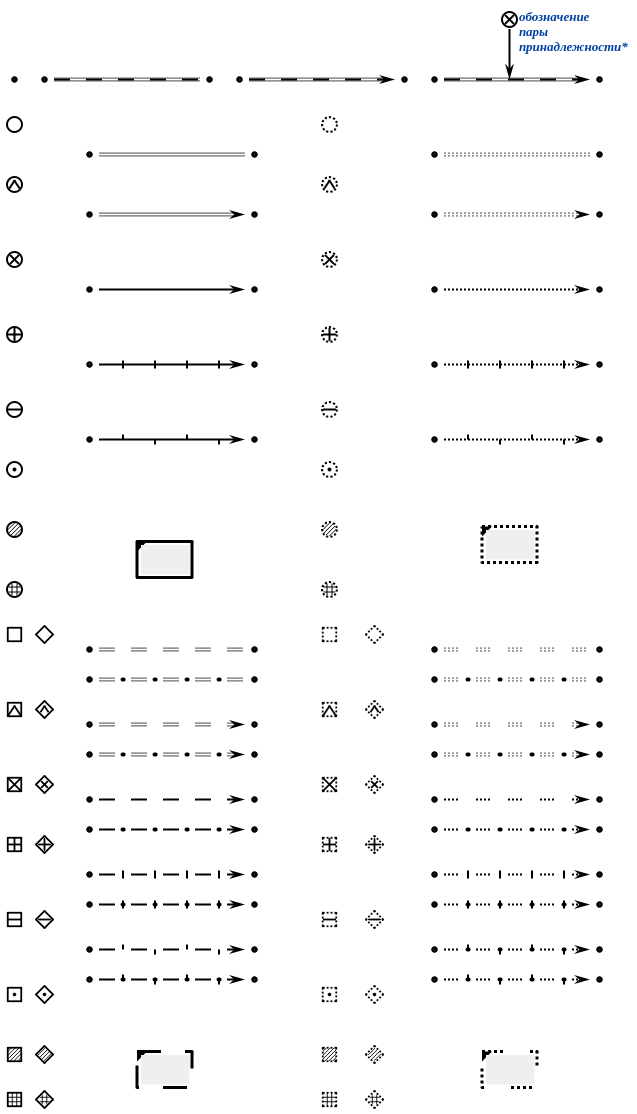
\includegraphics[scale=0.7]{images/intro/scg/SCg-full.png}
	\label{fig:scg_full}
\end{figure}

\bigskip
Трудно сразу поверить, что на основе такого простого алфавита можно построить удобный и \myuline{универсальный} \textit{графовый язык}. В рамках \textit{Документации Технологии OSTIS} мы постараемся Вас в этом убедить. Кроме того, нас не должна настораживать простота алфавита, поскольку человечество имеет большой опыт кодирования, хранения в памяти и передачи по каналам связи самых различных информационных ресурсов, используя алфавит, состоящий только из двух классов элементов --- единиц и нулей. 

Мы ведем речь о принципиально ином (графовом) способе кодирования информации в \textit{компьютерных системах}, но стараемся при этом свести это кодирование к достаточно простому алфавиту хотя бы для того, чтобы искусственно не усложнять проблему создания нового поколения компьютеров, основанных на указанном способе кодирования информации. 

Расширения \textit{Ядра SCg-кода} рассмотрим как направления перехода от текстов \textit{Ядра SCg-кода} к более компактным текстам. Но, поскольку это приводит к усложнению \textit{Синтаксиса SCg-кода} и, в первую очередь, к расширению \textit{Алфавита SCg-кода\scnsupergroupsign}, делать такие расширения необходимо обоснованно с учетом частоты встречаемости в рамках \textit{баз знаний ostis-систем} соответствующих фрагментов.

\subsection{Денотационная семантика SCg-кода}
\label{sec_scg_semantics}

В \textit{SCg-коде} выделяются Ядро SCg-кода и его расширения. 
\textbf{\textit{Алфавит Ядра SCg-кода\scnsupergroupsign}} --- алфавит \textit{sc.g-элементов}, графически изображаемых \textit{sc-элементов}. \textit{Алфавит Ядра SCg-кода\scnsupergroupsign} взаимно однозначно соответствует \textit{Алфавиту SC-кода\scnsupergroupsign}.

\textit{Денотационная семантика Ядра SCg-кода} соответствует \textit{Денотационной семантике SC-кода}. Это продемонстрировано в \textit{\nameref{fig:scg_core-alphabet}}.

\begin{figure}[H]
	\centering
	\caption{Таблица. Алфавит Ядра SCg-кода\scnsupergroupsign}
	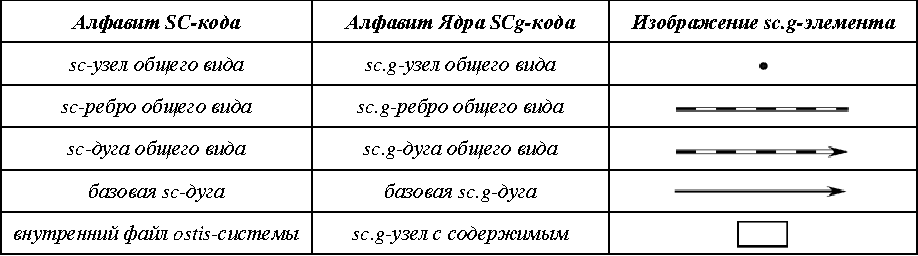
\includegraphics[scale=0.8]{images/intro/scg/SCg-core-alphabet.pdf}
	\label{fig:scg_core-alphabet}
\end{figure}

\textit{Алфавит Ядра SCg-кода\scnsupergroupsign} представлен следующими элементами:
\begin{textitemize}
	\item \textbf{\textit{sc.g-узел общего вида}} --- \textit{sc.g-элемент}, являющийся графическим изображением \textit{sc-узла общего вида}. Все \textit{sc-узлы}, не являющиеся знаками файлов, в тексте (конструкции) \textit{Ядра SCg-кода}, изображаются в виде небольших черных кругов одинакового диаметра, который обозначим через $\bm{d}$, и точная величина которого зависит от масштаба отображения \textit{sc.g-текста};
	
	\item \textbf{\textit{sc.g-ребро общего вида}} --- \textit{sc.g-элемент}, являющийся графическим изображением \textit{sc-ребра общего вида}. Каждое \textit{sc-ребро} в \textit{Ядре SCg-кода} изображается в виде широкой линии, в которой чередуются фрагменты со сплошной заливкой и без заливки, не имеющей самопересечений и имеющей общую толщину, равную примерно $\bm{0.7d}$;
	
	\item \textbf{\textit{sc.g-дуга общего вида}} --- \textit{sc.g-элемент}, являющийся графическим изображением \textit{sc-дуги общего вида}. Каждая \textit{sc-дуга} в \textit{Ядре SCg-кода} изображается в виде широкой линии, в которой чередуются фрагменты со сплошной заливкой и без заливки, не имеющей самопересечений, имеющей общую толщину, равную примерно $\bm{0.7d}$ и имеющей изображение стрелочки на одном из концов этой линии;
	
	\item \textbf{\textit{базовая sc.g-дуга}} --- \textit{sc.g-элемент}, являющийся графическим изображением \textit{базовой sc-дуги}. Каждая входящая в состав sc-текста \textit{базовая sc-дуга} в \textit{Ядре SCg--кода} изображается в виде линии произвольной формы, не имеющий самопересечений, имеющий толщину $\bm{0.4d}$, и имеющей изображение стрелочки на одном из ее концов;
	
	\item \textbf{\textit{внутренний файл ostis-системы}} --- \textit{sc-узел}, являющийся знаком \textit{внутреннего файла ostis-системы}, sc-знак \textit{внутреннего файла ostis-системы};
	
	\item \textbf{\textit{sc.g-узел с содержимым}} --- \textit{sc.g-узел}, имеющий содержимое, sc.g-узел, являющийся знаком внутреннего файла ostis-системы, sc.g-рамка. \textit{sc.g-рамка} --- это всегда прямоугольник, максимальный размер которого не ограничивается, но минимальный фиксируется и соответствует \textit{sc.g-рамке}, внутри которой обозначаемый ею \textit{файл} не отображается. Каждый входящий в sc-текст \textit{sc-узел, имеющий содержимое}, в \textit{Ядре SCg-кода} изображается в виде прямоугольника произвольного размера с толщиной линии $\bm{0.6d}$. Внутри этого прямоугольника отображается \textit{файл}, обозначаемый изображаемым \textit{sc-узлом}. Если нет необходимости изображать в тексте сам \textit{файл}, то \textit{sc-узел}, обозначающий такой \textit{файл}, в \textit{sc.g-тексте} изображается в виде прямоугольника со сторонами $\bm{2d}$ по вертикали и $\bm{4d}$ по горизонтали.
\end{textitemize}

\subsection{Иерархическое семейство подъязыков, семантически эквивалентных SCg-коду}
\label{sec_scg_extensions}

\begin{SCn}
\begin{scnrelfromlist}{ключевой знак}
	\scnitem{Первое направление расширения Ядра SCg-кода}
	\scnitem{Второе направление расширения Ядра SCg-кода}
	\scnitem{Третье направление расширения Ядра SCg-кода}
	\scnitem{Четвертое направление расширения Ядра SCg-кода}
	\scnitem{Пятое направление расширения Ядра SCg-кода}
	\scnitem{Шестое направление расширения Ядра SCg-кода}
	\scnitem{Седьмое направление расширения Ядра SCg-кода}
\end{scnrelfromlist}
\end{SCn}

\textbf{\textit{Первое направление расширения Ядра SCg-кода}}

\textit{Первое направление синтаксического расширения Ядра SCg-кода} --- это \myuline{приписывание} некоторым \mbox{sc.g-элементам} \textit{основных sc-идентификаторов*} (чаще всего --- строковых идентификаторов, то есть имен) \textit{sc-элементов} , изображаемых этими \textit{sc.g-элементами}. Указываемые идентификаторы являются уникальным для каждого идентифицируемого (именуемого) \textit{sc.g-элемента}. Приписывание \textit{sc.g-элементам} уникальных идентификаторов дает возможность в рамках одного \textit{sc.g-текста} дублировать (копировать) некоторые \textit{sc.g-узлы} при условии, если \myuline{всем} таким копиям будут приписаны соответствующие идентификаторы. Такое дублирование \textit{sc.g-узлов} является дополнительным средствам \myuline{наглядного} размещения \textit{sc.g-текстов}. Кроме того, приписывание \textit{sc.g-элементу} соответствующего ему основного (уникального) \textit{sc-идентификатора*} представляет собой более компактный вариант изображения \textit{sc.g-текстов}.

\begin{figure}[H]
	\centering
	\caption{Рисунок. Пример sc.g-текста, трансформируемого по Первому направлению расширения Ядра SCg-кода}
	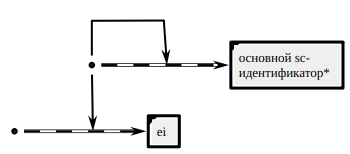
\includegraphics[scale=0.8]{images/intro/scg/scg_transf1.png}
	\label{fig:scg_example_1}
\end{figure}

Здесь (в левом нижнем углу приведенного sc.g-текста) представлен \textit{sc.g-узел общего вида}, изображающий \textit{sc-узел общего вида}, которому соответствует \textit{основной sc-идентификатор*} в виде строки ``\textbf{\textit{ei}}''.

\bigskip
\textit{sc.g-узлу общего вида} изображающему \textit{sc-узел}, внешним идентификатором которого является строка ``\textit{основной sc-идентификатор*}'' и который, соответственно является знаком \textit{бинарного ориентированного отношения}, каждая \textit{пара} которого связывает идентифицируемый \textit{sc-элемент} с его основным внешним sc-идентификатором, приписывается указанный внешний идентификатор изображаемого им \textit{sc-элемента}. Это продемонстрировано на  \textit{\nameref{fig:scg_transf_1}}.

\begin{figure}[H]
	\centering
	\caption{Рисунок. Трансформация sc.g-текста по Первому направлению расширения Ядра SCg-кода}
	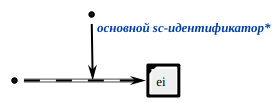
\includegraphics[scale=0.8]{images/intro/scg/scg_transf2.png}
	\label{fig:scg_transf_1}
\end{figure}


\bigskip
В результате данной трансформации исходный \mbox{\textit{sc.g-текст}} трансформируется в один \textit{sc.g-общего вида}, которому приписывается \textit{основной sc-идентификатор} ``\textit{\textbf{ei}}''. Это продемонстрировано на  \textit{\nameref{fig:scg_transf_2}}.

\begin{figure}[H]
	\centering
	\caption{Рисунок. Результат трансформации sc.g-текста по Первому направлению расширения Ядра SCg-кода}
	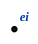
\includegraphics[scale=0.8]{images/intro/scg/scg_transf3.png}
	\label{fig:scg_transf_2}
\end{figure}

Подчеркнем, что рассматриваемая трансформация преобразует исходный текст Ядра \textit{SCg-кода} в текст, семантически эквивалентный, но принадлежащий не Ядру \textit{SCg-кода}, а его расширению.

\textbf{\textit{Второе направление расширения Ядра SCg-кода}}

\textit{Второе направление расширения Ядра SCg-кода} --- это уточнение типологии \textit{константных постоянных сущностей} и расширение \textit{Алфавита Ядра SCg-кода\scnsupergroupsign}, позволяющее типологию \textit{константных постоянных сущностей} привести в соответствие с синтаксической типологией новых вводимых элементов \textit{Алфавита SCg-кода\scnsupergroupsign}. Рассмотрим подробнее sc.g-элементы, знаки \textit{константных постоянных сущностей} различного вида. Графическим признаком \textit{константных постоянных sc-узлов} в конструкциях SCg-кода является их изображение в виде \myuline{окружностей} диаметра $3d$, где $d$ --- диаметр sc.g-узла общего вида. Такое изображение является более компактной записью факта принадлежности заданного sc-узла (назовем его $\bm{vi}$) классу sc-констант и классу обозначений постоянных сущностей. Запись этого факта в \textit{Ядре SCg-кода} потребует (1) явного изображения sc-узла, обозначающего класс всевозможных константных sc-элементов (класс \textit{sc-констант}), (2) явного изображения базовой sc-дуги, соединяющего изображение sc-узла, обозначающего класс sc-констант, с изображением заданного константного sc-узла, (3) явного изображение sc-узла, обозначающего класс всевозможных sc-элементов, обозначающих \textit{постоянные сущности}, (4) явного изображения базовой sc-дуги, соединяющего изображение sc-узла, обозначающего класс обозначений \textit{постоянных сущностей} с изображением рассматриваемого sc-узла $\bm{vi}$ (см. \textit{Файл. Изображение спецификации sc.g-элемента средствами Ядра SCg-кода и Первого расширения Ядра SCg-кода}).

\textit{Второе направление расширения Ядра SCg-кода} --- это уточнение типологии \textit{константных постоянных сущностей} и расширение \textit{Алфавита Ядра SCg-кода\scnsupergroupsign}, позволяющее типологию \textit{константных постоянных сущностей} привести в соответствие с синтаксической типологией новых вводимых элементов \textit{Алфавита SCg-кода\scnsupergroupsign}. Рассмотрим подробнее sc.g-элементы, знаки \textit{константных постоянных сущностей} различного вида. Графическим признаком \textit{константных постоянных sc-узлов} в конструкциях SCg-кода является их изображение в виде \myuline{окружностей} диаметра $3d$, где $d$ --- диаметр sc.g-узла общего вида. Такое изображение является более компактной записью факта принадлежности заданного sc-узла (назовем его $\bm{vi}$) классу sc-констант и классу обозначений постоянных сущностей. Запись этого факта в \textit{Ядре SCg-кода} потребует:
\begin{textitemize}
	\item явного изображения sc-узла, обозначающего класс всевозможных константных sc-элементов (класс \textit{sc-констант});  
	\item явного изображения базовой sc-дуги, соединяющего изображение sc-узла, обозначающего класс sc-констант, с изображением заданного константного sc-узла; 
	\item явного изображение sc-узла, обозначающего класс всевозможных sc-элементов, обозначающих \textit{постоянные сущности};
	\item явного изображения базовой sc-дуги, соединяющего изображение sc-узла, обозначающего класс обозначений \textit{постоянных сущностей} с изображением рассматриваемого sc-узла $\bm{vi}$ (см. \textit{Файл. Изображение спецификации sc.g-элемента средствами \textit{Ядра SCg-кода} и \textit{Первого расширения Ядра SCg-кода}}).
\end{textitemize}

\bigskip
Общепринятая запись данного факта выглядит следующим образом:

``\textit{sc-константа} $\ni \bm{vi}$; \textit{постоянная сущность} $\ni \bm{v_i};$''
\bigskip

\begin{textitemize}
	\item \textit{Константные постоянные sc-ребра} в конструкциях SCg-кода изображаются в виде двойной линии, каждая из которых имеет толщину примерно $d/7$, а расстояние между ними равно примерно $3d/7$. 
	\item \textit{Константные постоянные sc-дуги} изображаются в виде такой же двойной линии, но со стрелочкой. Все \textit{базовые sc-дуги}, а также все sc-узлы, имеющие содержимое, по определению являются \textit{константными постоянными sc-элементами}. 
	\item \textit{Константные sc.g-узлы}, изображаемые окружностями диаметра $3d$ и толщиной границы $d/5$, обозначают \textit{константные постоянные сущности}, о которых мало что известно, но известно то, что они не являются парами (то есть множествами, \textit{мощность*} которых равна 2) и, следовательно, не могут быть изображены в виде sc.g-дуг или sc.g-ребер. Но, если при этом об обозначаемой \textit{константной постоянной сущности} ($\bm{vi}$) известно, что она является классом сущностей, то явное указание принадлежности sc-элемента \textit{vi} всевозможных классов можно заменить на специальное графическое изображение sc-элемента \textit{vi}, предполагаемое указанную принадлежность. Это приводит к расширению  \textit{Алфавита SCg-кода\scnsupergroupsign} (см. \textit{Примеры sc.g-текстов, трансформируемых по Второму направлению расширения Ядра SCg-код}).
\end{textitemize}


Аналогичным образом вводятся: 
\begin{textitemize}
	\item \textit{sc.g-узел}, являющийся изображением \textit{класса};  
	\item \textit{sc.g-узел}, являющийся изображением \textit{класса классов};  
	\item \textit{sc.g-узел}, являющийся изображением \textit{отношения}; 
	\item \textit{sc.g-узел}, являющийся изображением \textit{ролевого отношения}; 
	\item \textit{sc.g-узел}, являющийся изображением \textit{структуры};  
	\item \textit{sc.g-узел}, являющийся изображением \textit{небинарной связки};
	\item \textit{sc.g-узел}, являющийся изображением \textit{первичной сущности} (терминальной сущности, которая не является множеством, а также файлом, хранимым в памяти ostis-системы).
\end{textitemize}

Важное место среди константных постоянных сущностей занимают \textit{константные постоянные пары принадлежности}, обозначаемое соответствующими \textit{sc.g-дугами}. Такие пары принадлежности и обозначающие их sc.g-дуги бывают позитивными, негативными и нечеткими. Константная постоянная позитивная sc.g-дуга принадлежности есть ничто иное, как \textit{базовая sc.g-дуга}. Константная постоянная негативная sc.g-дуга принадлежности изображается в виде \textit{базовой sc.g-дуги}, перечеркнутой штриховыми черточками. Константная постоянная нечеткая sc.g-дуга принадлежности изображается в виде \scnqqi{недочеркнутой} \textit{базовой sc.g-дуги}, с каждой стороны которой отображаются штрихи, по длине равные половине от длины штрихов, которыми перечеркнута \textit{константная постоянная негативная sc.g-дуга}.

\textbf{\textit{Третье направление расширения Ядра SCg-кода}}

\textit{Третье направление расширения Ядра SCg-кода} --- это расширение его алфавита путем введения дополнительных sc.g-элементов, обозначающих \textit{константные временные сущности} различного вида. Признаком sc.g-элементов, обозначающих \textit{константные временные сущности} являются точечные линии (линии, состоящие из точек, размер которых равен размеру изображаемой линии и которые близко расположены друг к другу на расстоянии, равном половине их размера), с помощью которых рисуются окружности при изображении sc-узлов, а также линии при изображении sc-коннекторов.

Результатом \textit{Третьего направления расширения Ядра SCg-кода} является введение следующих видов \textit{sc.g-элементов} (см. \textit{Примеры sc.g-текстов, трансформируемых по Третьему направлению расширения Ядра SCg-кода}).

\textbf{\textit{Четвертое направление расширения Ядра SCg-кода}}

\textit{Четвертое направление расширения Ядра SCg-кода} --- это расширение его алфавита путем введения дополнительных элементов, обозначающих \textit{переменные постоянные сущности} различного вида. Признаком sc.g-элементов, обозначающих сущности указанного класса, являются квадратики для изображения обозначений \textit{переменных постоянных сущностей}, не являющихся бинарными связями, а также пунктирные и штрих-пунктирные линии для изображения \textit{переменных постоянных бинарных связей}. 

Подчеркнем, что \textit{переменные постоянные сущности} могут отличаться друг от друга по характеру их \textit{области значений*}. Этими значениями в общем случае могут быть как \textit{константные постоянные сущности}, так и \textit{переменные постоянные сущности}. В любом случае, значение \textit{переменной сущности} является либо \textit{константной сущностью}, либо \textit{переменной сущностью}. Если каждое значение переменной является константой, то такую переменную будем называть \textit{переменной первого уровня}. Если каждое значение переменной является \textit{переменной первого уровня}, то такую переменную будем называть \textit{переменной второго уровня}. 

\textbf{\textit{переменная постоянная сущность первого уровня}} (первичная sc-переменная), не являющаяся бинарной связью --- это переменная, каждым значением которой является \textit{константная постоянная сущность}, не являющаяся бинарной связью. Такая переменная изображается квадратиком, который ориентирован по вертикали и горизонтали. 

\textit{переменная постоянная сущность второго уровня} (вторичная sc-переменная), не являющаяся бинарной связью, изображается квадратиком, повернутым на 45$^\circ$. 

Указанная выше семантика таких изображений приписывается \myuline{по умолчанию}. Это означает, что, если обозначаемая sc-переменная имеет более сложную структуру области ее значений (является sc-переменной третьего и выше уровня или sc-переменной, значения которой имеют различный логический уровень), то эта область должна быть специфицирована явно, при этом такая sc-переменная в SCg-коде изображается так же, как первичная sc-переменная.

\textbf{\textit{Пятое направление расширения Ядра SCg-кода}}
	
\textit{Пятое направление расширения Ядра SCg-кода} --- это расширение его алфавита путем введения дополнительных \textit{sc.g-элементов}, обозначающих \textit{переменные временные сущности} различного вида. Указанные дополнительные \textit{sc.g-элементы} аналогичны тем, которые введены в рамках \textit{Четвертого направления расширения Ядра SCg-кода}, и отличаются только тем, что в \textit{Пятом направлении расширении Ядра SCg-кода} речь идет о переменных \myuline{временных} сущностях, а в \textit{Четвертом направлении расширения Ядра SCg-кода} --- о переменных \myuline{постоянных} сущностях.

\textbf{\textit{Шестое направление расширения Ядра SCg-кода}}

\textit{Шестое направление расширения Ядра SCg-кода} --- это введение в SCg-код \textit{sc.g-контуров} и \textit{sc.g-шин} как средств структуризации sc.g-текстов и повышения наглядности при их размещении. Подчеркнем, что и sc.g-контуры, и sc.g-шины, и sc.g-рамки являются специальными видами sc.g-элементов. При этом sc.g-контуры и sc.g-рамки являются sc.g-ограничителями (ограничителями SCg-кода).

Каждый \textbf{\textit{sc.g-контур}} изображается (в 2D-модификации) в виде замкнутой ломаной линии со скругленными изломами, ограничивающей некоторый фрагмент sc.g-текста и обозначает множество всех \myuline{sc-элементов}, sc.g-изображения которых оказались внутри этого контура. Толщина указанной линии составляет примерно $\bm{0.4d}$, где \textbf{\textit{d}} --- диаметр \textit{sc.g-узла общего вида}.

Обозначение \textit{множества sc-элементов}, изображаемое \textit{sc.g-контуром}, может быть как константным, так и переменным. Соответственно этому линия, изображающая \textit{sc.g-контур} может быть: 

\begin{textitemize}
	\item сплошной непунктирной линией,
	\item точечной непунктирной линией,
	\item сплошной пунктирной линией,
	\item точечной пунктирной линией.
\end{textitemize}

\bigskip
Семантическим эквивалентом \textit{sc.g-контуру} является \textit{sc.g-узел, обозначающий структуру}. Использование \textit{sc.g-контура} вместо указанного \textit{sc.g-узла} исключает необходимость явно изображать \textit{sc-дуги принадлежности}, выходящие из этого \textit{sc.g-узла}. Это существенно повышает уровень наглядности \textit{sc.g-текста}.

Если представленный внутри \textit{sc.g-контура} текст не является \textit{sc.g-текстом}, то считается, что на самом деле внутренностью \textit{sc.g-контура} является \textit{sc.g-текст}, являющийся результатом перевода предоставленного текста в \textit{SCg-код}.

Каждая \textbf{\textit{sc.g-шина}} представляет собой замкнутую или незамкнутую линию толщиной примерно равной диаметру \textit{sc.g-узла общего вида}, которая инцидентна только одному \textit{sc.g-элементу} и семантически ему эквивалентна. Идея введения \textit{sc.g-шин} заключается в увеличении «размеров» \textit{sc.g-элементов} для расширения их области инцидентности. Особенно актуально это для \textit{sc.g-узлов}, имеющих большое число инцидентных им \textit{sc.g-коннекторов}.

\bigskip
\textbf{\textit{Седьмое направление расширения Ядра SCg-кода}}
	
\textit{Седьмое направление синтаксического расширения Ядра SCg-кода} --- это переход от 2D-изображений \textit{sc.g-текстов} к 3D-изображениям.

Одним из вариантов трехмерного изображения \textit{sc.g-текстов} является следующий:
\begin{textitemize}
	\item все sc.g-узлы изображаются, как и ранее, \myuline{плоскими} графическими примитивами. При изменении точки просмотра они \myuline{всегда} \scnqqi{поворачиваются} параллельно плоскости экрана, но их масштаб (размер на экране) при удалении от точки просмотра \myuline{уменьшается};
	\item аналогичным \scnqqi{плоским} образом изображаются \textit{sc.g-рамки} с их \scnqqi{внутренним} содержанием, а также внешние идентификаторы, приписываемые \textit{sc.g-элементам};
	\item \textit{sc.g-коннекторы} изображаются \myuline{непересекающимися} линиями в трехмерном пространстве (заметим, что при изображении \textit{sc.g-текстов} на плоскости пересечение \textit{sc.g-коннекторов} часто снижает наглядность, \scnqqi{читабельность} \textit{sc.g-текстов}). Т.е. \textit{sc.g-коннекторы}, которые на плоскости изображаются двойными линиями, в пространстве  цилиндрическими, \scnqqi{трубчатыми линиями} с находящейся внутри тонкой, но просвечивающейся осевой линией;
	\item \textit{sc.g-контур} в пространстве визуализируется несколькими (!) специального вида точками --- например там, где есть точки инцидентности \textit{sc.g-контура} с \myuline{внешними} \textit{sc.g-коннекторами}. При этом \textit{sc.g-контур} становится виден только по команде просмотра указываемого контура (указание контура --- это указание одной из его точек инцидентности). По этой команде цветом выделяются все граничные точки контура (точки инцидентности) и все внутренние \textit{sc.g-элементы} контура. Если просматривается  несколько контуров, то используется несколько цветов.
\end{textitemize}

Вторым вариантом 3D-визуализации \textit{sc.g-текстов} является размещение \textit{sc.g-текстов} на параллельных плоскостях (слоях) с “прошивками”\ между этими слоями, соединяющими синонимичные \textit{sc.g-узлы}, то есть \textit{sc.g-узлы}, имеющие одинаковые приписываемые им внешние идентификаторы. Такой вариант плоской, но многослойной визуализации \textit{sc.g-текстов} дает возможность широко использовать те средства просмотра и редактирования \textit{sc.g-текстов}, которые разработаны для плоской их визуализации(см. \scncite{Standart2021}).

\section{Язык внешнего линейного представления конструкций SC-кода --- SCs-код (Semantic Code string)}
\markboth{Язык внешнего линейного представления конструкций SC-кода --- SCs-код}{Язык внешнего линейного представления конструкций SC-кода --- SCs-код}
\label{sec_scs}

\begin{SCn}
\begin{scnrelfromlist}{подраздел}
	\scnitem{\ref{sec_scs_syntax}~\nameref{sec_scs_syntax}}
	\scnitem{\ref{sec_scs_semantics}~\nameref{sec_scs_semantics}}
	\scnitem{\ref{sec_scs_extensions}~\nameref{sec_scs_extensions}}
\end{scnrelfromlist}

\bigskip

\begin{scnrelfromlist}{ключевой знак}
	\scnitem{SCs-код}
	\scnitem{Алфавит SCs-кода\scnsupergroupsign}
	\scnitem{Синтаксис SCs-кода}
	\scnitem{Денотационная семантика SCs-кода}
	\scnitem{Иерархическое семейство подъязыков, семантически эквивалентных SCs-коду}
\end{scnrelfromlist}

\begin{scnrelfromlist}{ключевое понятие}
	\scnitem{sc.s-предложение}
	\scnitem{sc.s-ограничитель}
	\scnitem{sc.s-разделитель}
	\scnitem{sc.s-модификатор}
	\scnitem{sc.s-элемент}
	\scnitem{sc.s-коннектор}
	\scnitem{sc.s-ребро}
	\scnitem{sc.s-дуга}
\end{scnrelfromlist}
\end{SCn}

\subsection*{Введение в \ref{sec_scs}}

\begin{SCn}
\scnheader{SCs-код}
\scnidtf{Semantic Code string}
\scnidtf{Язык линейного представления знаний ostis-систем}
\scnidtf{Множество всевозможных текстов \textit{SCs-кода}}
\scnidtf{Язык внешнего линейного представления конструкций внутреннего языка ostis-систем}
\end{SCn}

\textbf{\textit{SCs-код}} представляет собой множество линейных текстов (\textit{sc.s-текстов}), каждый из которых состоит из предложений (\textit{sc.s-предложений}), разделенных друг от друга двойной \textit{точкой с запятой} (разделителем \textit{sc.s-предложений}). При этом \mbox{\textit{sc.s-предложение}} представляет собой последовательность \textit{sc-идентификаторов}, являющихся именами описываемых \textit{сущностей} и разделяемых между собой различными \textit{sc.s-разделителями} и \textit{sc.s-ограничителями}.

\subsection{Синтаксис SCs-кода}
\label{sec_scs_syntax}

\begin{SCn}
	\scnheader{Алфавит SCs-кода\scnsupergroupsign}
	\scnidtf{Алфавит символов SCs-кода\scnsupergroupsign}
	\scnidtf{множество символов SCs-кода}
	\scnidtf{символ, используемый в текстах SCs-кода}
	\scnidtf{Язык внешнего линейного представления информационных конструкций
		внутреннего языка ostis-систем}
	\begin{scnreltoset}{объединение}
		\scnitem{Алфавит символов, используемых в sc.s-разделителях\scnsupergroupsign}
		\scnitem{Алфавит символов, используемых в sc.s-ограничителях\scnsupergroupsign}
		\scnitem{Алфавит символов, используемых в sc-идентификаторах\scnsupergroupsign}
		\begin{scnindent}
			\begin{scnreltoset}{объединение}
				\scnitem{Алфавит символов, используемых в простых строковых sc-идентификаторах\scnsupergroupsign}
				\scnitem{Алфавит символов, используемых в sc-выражениях\scnsupergroupsign}			
			\end{scnreltoset}
		\end{scnindent}
		\scnitem{Алфавит символов, используемых в неоднозначных sc.s-изображениях sc-узлов\scnsupergroupsign}
	\end{scnreltoset}
\end{SCn} 

\textbf{\textit{Алфавит SCs-кода\scnsupergroupsign}} строится на основе современных общепринятых наборов символов, что позволяет упростить разработку средств для работы с \textit{sc.s-текстами} с использованием современных технологий.

В состав \textit{sc.s-текстов}, как и в состав текстов любых других языков, являющихся вариантами внешнего отображения текстов \textit{SC-кода}, могут входить различные файлы, в том числе естественно-языковые или даже файлы, содержащие другие \textit{sc.s-тексты}. В общем случае в таких файлах могут использоваться самые разные символы, в связи с чем будем считать, что в \textit{Алфавит SCs-кода\scnsupergroupsign} эти символы не включаются.

\textbf{Алфавит символов, используемых в \textit{sc.s-разделителях}\scnsupergroupsign} состоит из: пробел, точка с запятой, двоеточие, круглый маркер и знак равенства.

\textbf{Алфавит символов, используемых в \textit{sc.s-разделителях}\scnsupergroupsign}, изображающих связь инцидентности sc-элементов, состоит из: `` < ''{}, `` > ''{}, `` | ''{}, `` - ''{}.

\textbf{Базовый алфавит символов, используемых в \textit{sc.s-коннекторах}\scnsupergroupsign} состоит из: `` $\sim$ ''{}, знак подчеркивания, знак равенства, двоеточие, `` < ''{}, `` > ''{}, `` --- ''{}, `` | ''{}, `` / ''{}.
	
\textbf{Расширенный алфавит символов, используемых в \textit{sc.s-коннекторах}\scnsupergroupsign} состоит из:
	``$\in$''{}, 
	``$\ni$''{}, ``$\subseteq$''{}, ``$\supseteq$''{},   ``$\subset$''{}, ``$\supset$''{}, ``$\leq$''{},  ``$\geq$''{}, ``$\Leftarrow$''{}, ``$\Rightarrow$''{}, ``$\leftarrow$''{}, ``$\rightarrow$''{}, 
	``$\Leftrightarrow$''{}.


При необходимости комбинации указанных признаков перечисленные символы комбинируются так, как показано в параграфе \scnqqi{\textit{Описание sc.s-разделителей и sc.s-ограничителей}}.

Как в \textit{Базовом}, так и в \textit{Расширенном Алфавитах} \textit{sc.s-коннекторов} используются следующие общие признаки, характеризующие тип изображаемого \textit{sc-коннектора}:
\begin{textitemize}
	\item знак подчеркивания как признак изображений переменных \textit{sc-коннекторов} (один знак подчеркивания для \textit{sc-коннекторов}, являющихся первичными \textit{sc-переменными}, два знака подчеркивания для \textit{sc-коннекторов}, являющихся вторичными \textit{sc-переменными (sc-метапеременными)});
	\item вертикальная черта \scnqqi{ $ | $ } как признак изображений \textit{негативных sc-дуг принадлежности};
	\item косая черта \scnqqi{ $ / $ } как признак изображений \textit{нечетких sc-дуг принадлежности};
	\item тильда \scnqqi{ $ \sim $ } как признак изображений \textit{временных sc-дуг принадлежности}.
\end{textitemize}

Для упрощения процесса разработки исходных текстов \textit{баз знаний} с использованием \textit{SCs-кода} и создания соответствующих средств вводятся два алфавита символов(см. \nameref{fig:scs_membership_connectors1}). \textit{Базовый алфавит символов, используемых в sc.s-коннекторах\scnsupergroupsign} включает только символы, входящие в переносимый набор символов и имеющиеся на стандартной современной клавиатуре. Таким образом, для разработки исходных текстов баз знаний, использующих только \textit{Базовый алфавит символов, используемых в sc.s-коннекторах\scnsupergroupsign} достаточно обычного текстового редактора. \textit{Расширенный алфавит символов, используемых в sc.s-коннекторах\scnsupergroupsign} включает также дополнительные символы, которые позволяют сделать sc.s-тексты (и sc.n-тексты) более читабельными и наглядными. Для визуализации и разработки sc.s-текстов с использованием расширенного алфавита требуется наличие специализированных средств.

\begin{figure}[H]
	\centering
	\caption{Таблица. Описание изображения sc.s-коннекторов в Базовом и Расширенном алфавите SCg-кода\scnsupergroupsign}
	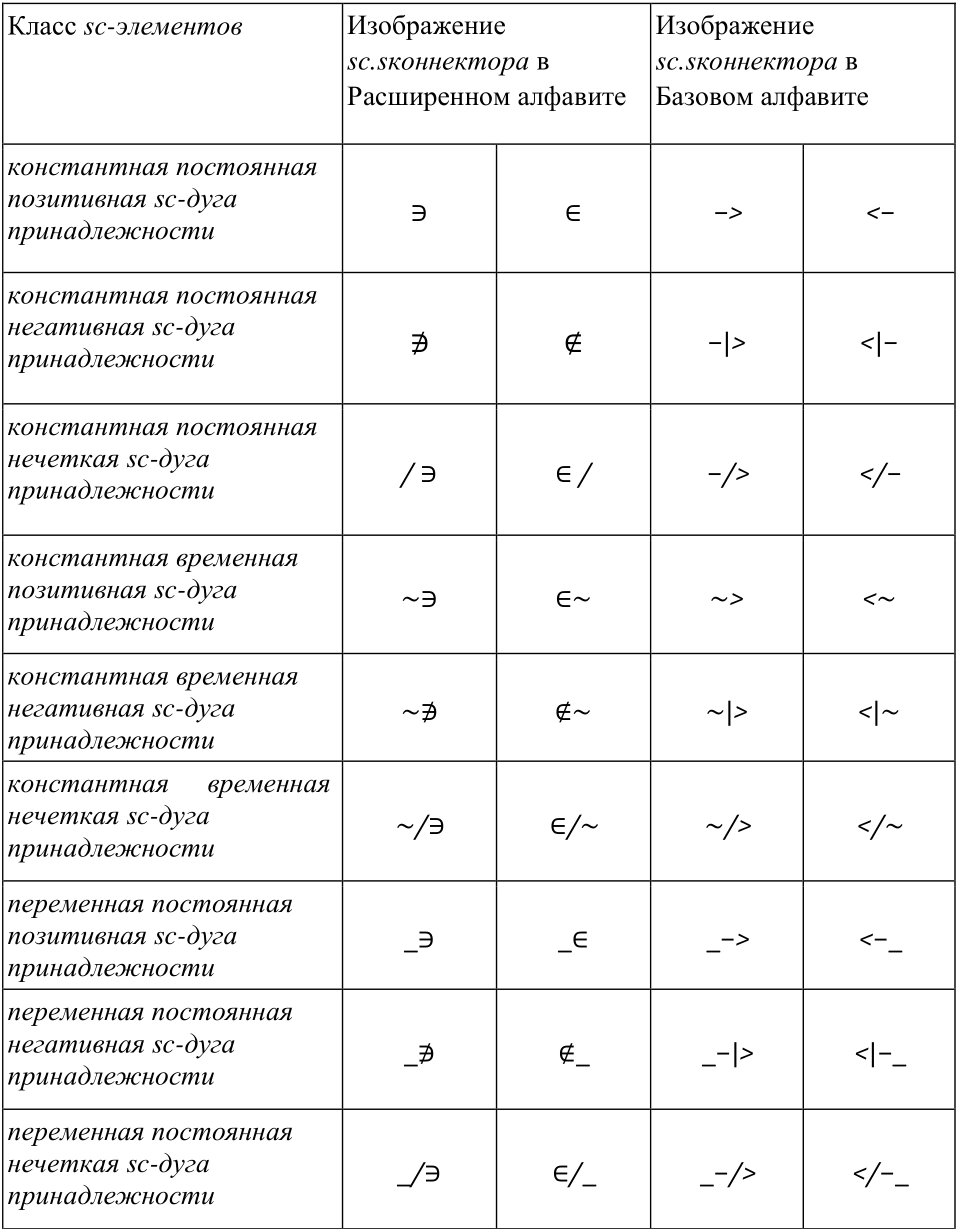
\includegraphics[scale=0.45]{images/intro/scs/scs_membership_connectors_01.png}
	\label{fig:scs_membership_connectors1}
\end{figure}

\newpage
\begin{figure}[H]
	\centering
	\caption{Таблица. Описание изображения sc.s-коннекторов в Базовом и Расширенном алфавите SCg-кода\scnsupergroupsign{} (продолжение)}
	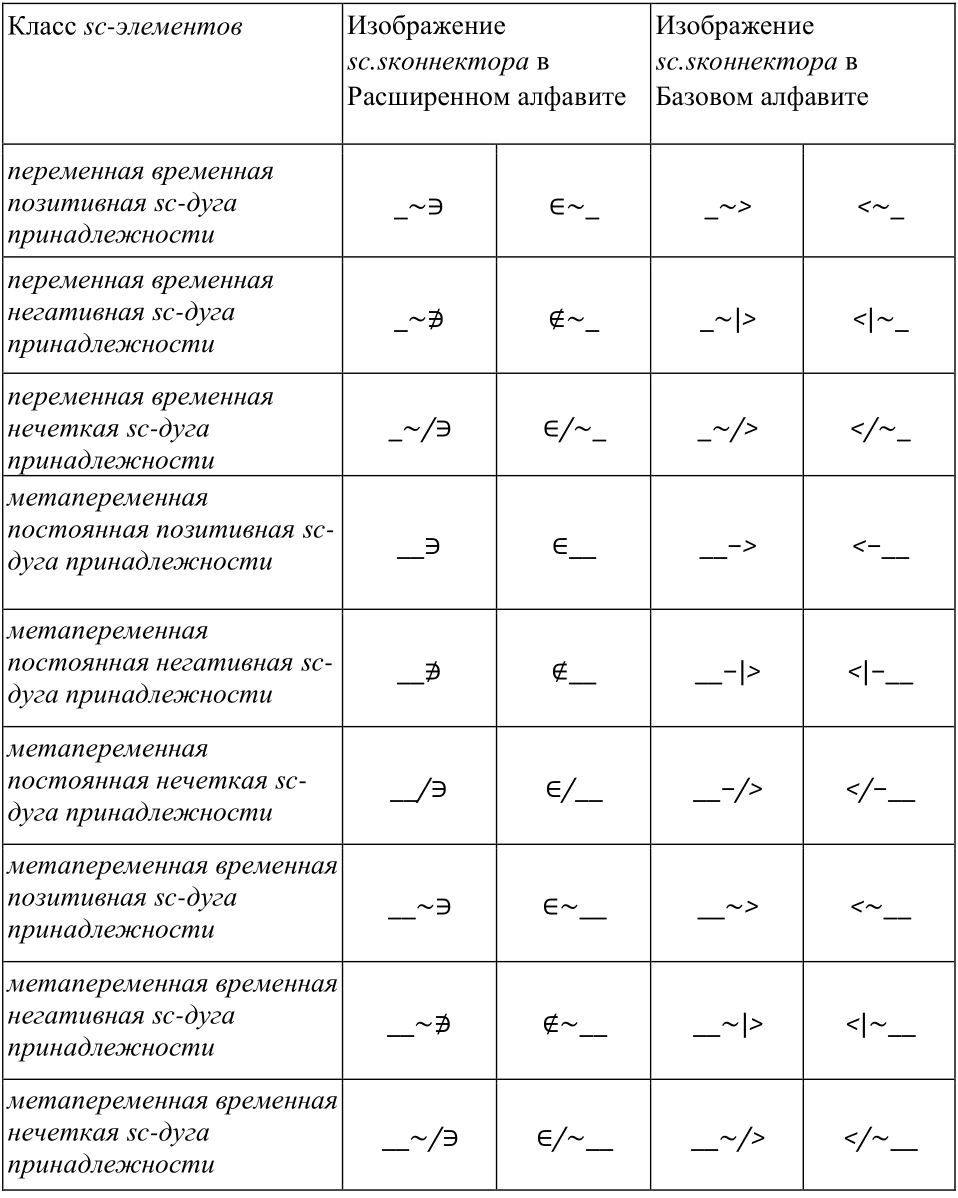
\includegraphics[scale=0.45]{images/intro/scs/scs_membership_connectors_02.png}
	\label{fig:scs_membership_connectors2}
\end{figure}

\textbf{Алфавит символов, используемых в \textit{sc.s-ограничителях}\scnsupergroupsign} состоит из: ``( ''{}, ``)''{}, ``*''{}.

\textbf{Алфавит символов, используемых в неоднозначных \textit{sc.s-изображениях sc-узлов}\scnsupergroupsign} состоит из:
``\{''{}, ``\}''{}, 
``-''{}, ``!''{}, ``~[ \,''{}, ``~] \,{}.

\bigskip
\textbf{\textit{Описание sc.s-разделителей и sc.s-ограничителей}}

\textbf{\textit{sc.s-разделитель}} и \textbf{\textit{sc.s-ограничитель}} являются важными элементами \textit{SCs-кода}.

Существует \textit{sc.s-разделитель}, используемый для структуризации \textit{sc.s-предложений} и \textit{sc.s-разделитель} \textit{sc.s-предложений}.

\textit{sc.s-разделить} --- разделитель, используемый в \textit{sc.s-текстах}. \textit{sc.s-разделитель} разбивается на:
\begin{textitemize}
	\item \textit{sc.s-разделитель}, используемый для структуризации \textit{\textit{sc.s-предложений}}.
	\begin{textitemize}
		\item Разделяет \textit{sc-идентификатор бинарного отношения} и второй компонент одной из связок этого отношения в случае, если указанное бинарное отношение и его связка связаны \textit{константной sc-дугой принадлежности}. Представляется в виде двоеточия.
		\item Разделяет \textit{sc-идентификатор бинарного отношения} и второй компонент одной из связок этого отношения в случае, если указанное бинарное отношение и его связка связаны \textit{переменной sc-дугой принадлежности}. Представляется в виде двойного двоеточия.
	\end{textitemize}
	\item \textit{sc.s-разделитель \textit{sc.s-предложений}}, представляется в виде двойной точки с запятой.    
\end{textitemize}

\bigskip
\textbf{\textit{sc.s-ограничитель}} представляется в виде: $(![  (\ast ]! \cup ![  \ast) ]!)$

Круглые скобки со звездочкой ограничивают присоединенные \textit{sc.s-предложения}, которые, в свою очередь, могут иметь в своем составе другие присоединенные \textit{sc.s-предложения}.

Также существует \textbf{\textit{sc.s-коннектор}}. Типология \textit{sc.s-коннекторов} полностью соответствует типологии \textit{sc.g-коннекторов}, и, тем более, \textit{sc-коннекторов}, так как она учитывает устоявшиеся традиции изображения связок целого ряда конкретных отношений.

\begin{SCn}
\scnheader{sc.s-коннектор}
\scnidtf{изображение \textit{sc-коннектора} во внешнем тексте SCs-кода или SCn-кода}
\scnsubset{sc.s-разделитель}
\end{SCn}

Выделяют следующие \textit{sc.s-коннекторы}:
\begin{textitemize}
	\item \textit{ориентированный \textit{sc.s-коннектор}},
	\item \textit{неориентированный \textit{sc.s-коннектор}};
	\item \textit{\textit{sc.s-коннектор}}, соответствующий \textit{sc.g-дуге принадлежности},
	\item \textit{\textit{sc.s-коннектор}}, соответствующий \textit{sc.g-коннектору}, который не является \textit{sc.g-дугой}.
\end{textitemize}

Типология \textit{sc.s-коннекторов} полностью соответствует типологии \textit{sc.g-коннекторов}, и, тем более, \textit{sc-коннекторов}, так как она учитывает устоявшиеся традиции изображения связок целого ряда конкретных отношений.

На множестве \textit{sc-элементов} задано бинарное ориентированное отношение инцидентности sc-элементов, а так же подмножество этого отношения --- отношение инцидентности входящих \textit{sc-дуг}, каждая пара которого связывает sc-дугу с тем sc-элементом, в который она входит. В \textit{SC-коде} \textit{sc-коннекторы} могут соединять между собой не только \textit{sc-узел} с \textit{sc-узлами}, но и \textit{sc-узел} с \textit{sc-коннектором} и даже \textit{sc-коннектор} с \textit{sc-коннектором}. В последнем случае, указывая инцидентность sc-коннекторов, необходимо уточнить, какой из них является соединяемым (связываемым), а какой-соединяющим (связующим). Поэтому отношение инцидентности, заданное на множестве sc-элементов является ориентированным. Первый компонент пары этого отношения – связующий \textit{sc-коннектор}, а второй --- связуемый \textit{sc-элемент}. Очевидно, что связующий \textit{sc-элемент} всегда является \textit{sc-коннектором}, а \textit{sc-узел} может быть только связуемым.

\textit{sc.s-разделитель}, изображающий связь инцидентности \textit{sc-элементов} разбивается на:
\begin{textitemize}
	\item знак инцидентности “правого” \textit{sc-коннектора} --- знак инцидентности \textit{sc-коннектора}, \textit{sc-идентификатор} которого находится справа, изображается в виде `` $ \vdash$ ''{};
	\item знак инцидентности “левого” \textit{sc-коннектора} --- знак инцидентности \textit{sc-коннектора}, \textit{sc-идентификатор} которого находится слева, изображается в виде `` $ \dashv$ ''{};
	\item знак инцидентности входящей \textit{sc-дуги} справа --- знак инцидентности \textit{sc-дуги}, \textit{sc-идентификатор} который находится справа, изображается в виде `` $ |<$ ''{};
	\item знак инцидентности входящей \textit{sc-дуги} слева --- знак инцидентности \textit{sc-дуги}, \textit{sc-идентификатор} который находится слева, изображается в виде `` $ >| $ ''{}.
\end{textitemize}

\begin{SCn}
\scnheader{sc.s-разделитель, изображающий связь инцидентности sc-элементов}
\begin{scnrelfromset}{разбиение}
	\scnitem{знак инцидентности “правого” sc-коннектора}
	\begin{scnindent}
		\scnidtf{знак инцидентности sc-коннектора, sc-идентификатор которого находится справа}
		\scneqfileclass{|-}
	\end{scnindent}
	\scnitem{знак инцидентности “левого” sc-коннектора}
	\begin{scnindent}
		\scnidtf{знак инцидентности sc-коннектора, sc-идентификатор которого находится слева}
		\scneqfileclass{-|}
	\end{scnindent}
	\scnitem{знак инцидентности входящей sc-дуги справа}
	\begin{scnindent}
		\scnidtf{знак инцидентности sc-дуги, sc-идентификатор который находится справа}
		\scneqfileclass{|<}
	\end{scnindent}
	\scnitem{знак инцидентности входящей sc-дуги слева}
	\begin{scnindent}
		\scnidtf{знак инцидентности sc-дуги, sc-идентификатор который находится слева}
		\scneqfileclass{>|}
	\end{scnindent}
\end{scnrelfromset}
\end{SCn}

Указанные \textit{sc.s-разделители} с точки зрения синтаксической структуры \textit{sc.s-предложений} аналогичны \textit{sc.s-коннекторам}, но с точки зрения их денотационной семантики в отличие от \textit{sc.s-коннекторов} они не являются изображениями соответствующих sc-коннекторов.

Знак равенства является \textit{sc.s-разделителем} двух \textit{sc-идентификаторов}, которые идентифицируют (именуют) одну и ту же сущность и, соответственно, являются \textit{sc-идентификаторами*} (внешними уникальными изображениями) одного и того же \textit{sc-элемента}. При этом из указанных двух \textit{sc-идентификаторов} чаще всего один является простым \textit{sc-идентификатором}, а второй --- \textit{sc-выражением}. Реже оба эти \textit{sc-идентификатора} являются \textit{sc-выражениями}. И совсем редко оба они являются \textit{простыми sc-идентификаторами}. Последнее обозначает то, что оба эти \textit{sc-идентификатора} являются основными \textit{sc-идентификаторами*} одного и того же \textit{sc-элемента}. 

Пример:
\textit{SC-код} = sc.s-текст;;

Здесь первый \textit{sc-идентификатор} является \textit{именем собственным}, а второй --- \textit{именем нарицательным}.

При трансляции \textit{sc.s-текста} в \textit{SC-код} знаку равенства на некотором этапе может быть поставлено в соответствие \textit{sc-ребро}, принадлежащее отношению \textit{синонимии}* \textit{sc-элементов}, идентифицируемых \mbox{\textit{sc-идентификаторами}}, связанными знаком равенства. Но на последующем этапе указанное \textit{sc-ребро} \myuline{удаляется}, а связанные им \textit{sc-элементы} \myuline{склеиваются}. Таким образом \textit{sc-ребро}, принадлежащее отношению \textit{синонимии}* \textit{sc-элементов}, имеет не только \textit{денотационную}, но и \textit{операционную семантик}у.

Знак равенства с включением --- изображение \textit{sc-дуги}, принадлежащей отношению погружения*, связывающей два \textit{sc-узла}, обозначающих \textit{sc-тексты}, первый из которых является погружающим, а второй (в который указанная \textit{sc-дуга} входит) является погружаемым, вводимым в состав первого \textit{sc-текста}. 

\textit{sc-дуга}, принадлежащая отношению погружения*, интерпретируется как команда погружения одного sc-текста в состав другого. При выполнении этой команды (1) все sc-элементы погружаемого \textit{sc-текста} становятся элементами, принадлежащими погружающему sc-тексту, (2) все синонимичные \textit{sc-элементы}, оказавшиеся в составе погружающего \textit{sc-текста}, склеиваются, (3) \textit{sc-узел}, обозначающий погружаемый \textit{sc-текст}, а так же спецификация этого \textit{sc-текста} (включая перечень всех его \textit{sc-элементов}) погружается в историю эволюции базы знаний вместе со спецификацией события погружения рассматриваемого \textit{sc-текста} в состав базы знаний.

Указанные \textit{sc.s-коннекторы} отличаются от остальных \textit{sc.s-коннекторов} тем, что они и соответствующие им \textit{sc-коннекторы} (\textit{sc-ребра}, принадлежащих отношению синонимии \textit{sc-элементов} и \textit{sc-дуги}, принадлежащие отношению погружения одного \textit{sc-текста} в состав другого) имеют не только \textit{денотационную}, но и \textit{операционную семантику}, так как являются командами склеивания и командами погружения.

\bigskip
\textbf{\textit{Описание sc.s-предложений}}

\begin{SCn}
\scnheader{sc.s-предложение}
\scnidtf{минимальный семантически целостный фрагмент sc.s-текста}
\scnidtf{минимальный sc.s-текст}
\end{SCn}

\textit{sc.s-предложение}, (1) \myuline{состоящее} или из двух \textit{sc-идентификаторов}, соединенных между собой \textit{\mbox{sc.s-коннектором}}, или из трех \textit{sc-идентификаторов}, разделенных \textit{sc.s-разделителями, изображающими связь инцидентности sc-элементов}, и (2) завершающееся \textit{двойной точкой с запятой}.

Нетрудно заметить, что \textit{простые sc.s-предложения} по сути аналогичны триплетам языка RDF (\mbox{RDF-триплетам}), за тем исключением, что \textit{простое sc.s-предложение} можно \scnqqi{развернуть} при помощи \textit{Операции конверсии sc.s-предложений*} не меняя при этом его смысл, а RDF-триплет нельзя. Это является одной из причин, по которой, в отличие от RDF-триплетов, в простых \mbox{sc.s-предложениях} \textit{\mbox{sc.s-коннекторы}} и \textit{\mbox{sc.s-разделители}, изображающие связь инцидентности \mbox{sc-элементов}} не могут быть опущены, поскольку они в том числе показывают направление изображаемой ими связи между sc-элементами.

Признаком завершения любого \textit{sc.s-предложения}, то есть последними его символами является \textit{двойная точка с запятой}, которую, следовательно, можно считать разделителем \textit{sc.s-предложений}.

Выделяют следующие операции над sc.s-предложениями:
\begin{textitemize}
	\item \textbf{\textit{Операция конверсии sc.s-предложения*}}
	
		Каждое \textit{sc.s-предложение} (в том числе, и \textit{простое sc.s-предложение}) можно преобразовать в семантически эквивалентное ему \textit{sc.s-предложение} путем конверсии (\scnqqi{разворота}) цепочки компонентов \textit{sc.s-предложения}. Так, например, при конверсии (\scnqqi{развороте}) простого \textit{\mbox{sc.s-предложения}} (1) первый его \textit{\mbox{sc-идентификатор}} (первый компонент этого \textit{\mbox{sc.s-предложения}}) становится третьим компонентом конвертированного \textit{ \mbox{sc.s-предложения}}, (2) второй его \textit{\mbox{sc-идентификатор}} (третий компонент исходного \textit{\mbox{sc.s-предложения}}) становится первым компонентом \scnqqi{конвертированного} \textit{\mbox{sc.s-предложения}} и (3) второй компонент исходного \textit{\mbox{sc.s-предложения}} (\textit{\mbox{sc.s-коннектор}} или \textit{\mbox{sc.s-разделитель}, изображающий связь инцидентности \mbox{sc-элементов}}, соединяющий указанные выше компоненты) остается вторым компонентом конвертированного \textit{\mbox{sc.s-предложения}}, но меняет направленность (\scnqqi{$\ni$} заменяется на \scnqqi{$\in$} и наоборот, \scnqqi{$\supset$} на \scnqqi{$\subset$} и наоборот, \scnqqi{$\Rightarrow$} на \scnqqi{$\Leftarrow$} и наоборот и так далее).
	
	\item \textbf{\textit{Операция присоединения sc.s-предложения*}}
		
		Операция соединения двух \textit{sc.s-предложений} при совпадении последнего компонента первого предложения с первым компонентом второго.
		В результате выполнения данной операции:
		\begin{textitemize}
			\item первый компонент второго \textit{sc.s-предложения} удаляется;
			\item оставшаяся часть второго предложения окружается \textit{sc.s-ограничителем} присоединенных предложений ("(*"{} и "*)"{}). Разделитель \textit{sc.s-предложений} (";;"{}) также попадает внутрь указанного ограничителя;
			\item полученная конструкция помещается между последним компонентом первого предложения и разделителем \textit{sc.s-предложений}, которым заканчивалось первое предложение;
			\item второе предложение, таким образом, становится \textit{присоединенным sc.s-предложением}.
		\end{textitemize}
	
		Аналогичным образом к любому присоединенному \textit{sc.s-предложению} могут "пристыковываться"\ другие присоединенные \textit{sc.s-предложения}, в общем случае уровень такой вложенности не ограничен.
		
		Присоединенные \textit{sc.s-предложения} используются для того, чтобы продолжить спецификацию какого-либо sc-элемента, \textit{sc-идентификатор} которого является последним компонентом в рамках какого-либо sc.s-предложения, не начиная при этом нового \textit{sc.s-предложения} и, таким образом, не дублируя указанный \mbox{sc-идентификатор}. Внутрь присоединенных sc.s-предложений также могут встраиваться другие присоединенные \textit{sc.s-предложения}, в общем случае уровень вложенности таких предложений не ограничен. Таким образом присоединенные \textit{sc.s-предложения} описывают "ветвление"{} \textit{sc.s-предложений}, при этом точками такого "ветвления"{} выступают \textit{sc-идентификаторы}, входящие в состав этих \textit{sc.s-предложений}.
		
		Благодаря введению \textit{присоединенных sc.s-предложений} появляется возможность любой \textit{sc-текст} изобразить в виде одного \textit{sc.s-предложения}, содержащего необходимое количество \textit{присоединенных sc.s-предложений}. Таким образом, \textit{SCs-код} по выразительной мощности становится эквивалентным \textit{SCn-коду}.
	
	\item \textbf{\textit{Операция слияния sc.s-предложений*}}
		
		Операция присоединения \textit{простого sc.s-предложения} к \textit{sc.s-предложению}, у которого последний sc.s-коннектор совпадает с \textit{sc.s-коннектором} \textit{простого sc.s-предложения}, а предшествующий указанному \textit{sc.s-коннектору} sc-идентификатор совпадает с первым sc-идентификатором простого sc.s-предложения.
		
		В результате выполнения этой операции совпадающие \textit{sc-идентификаторы} и \textit{sc.s-коннекторы} соединяемых \textit{sc.s-предложений} "склеиваются"{} , а последние \textit{sc-идентификаторы} соединяемых \textit{sc.s-предложений} становятся последними компонентами объединенного \textit{sc.s-предложения},
		разделенными \textit{точкой с запятой}. Аналогичным образом можно присоединять сколько угодно простых \textit{sc.s-предложений}.
	
	\item \textbf{\textit{Операция разложения sc.s-предложений на простые sc.s-предложения*}}
		
		Каждое \textit{sc.s-предложение} можно разложить на множество \textit{простых sc.s-предложений}, то есть представить в виде последовательности \textit{простых sc.s-предложений}.
	
	\item \textbf{\textit{Операция разложения sc.s-предложений на простые sc.s-предложения с sc.s-разделителем, изображающим связь инцидентности sc-элементов*}}
		
		Каждое \textit{sc.s-предложение} (в том числе и \textit{простое sc.s-предложение} с \textit{sc.s-коннектором}) можно представить в виде семантически эквивалентной последовательности \textit{простых \mbox{sc.s-предложений}} с \textit{sc.s-разделителем, изображающим связь инцидентности \mbox{sc-элементов}}.
		
		Данная операция осуществляет \myuline{однозначное} (!) формирование множества \textit{простых \mbox{sc.s-предложений}} указанного вида.
\end{textitemize}

Операции, заданные на множестве \textit{sc.s-предложений} можно разделить на три группы:
\begin{textitemize}
	\item группа операций конверсии \textit{sc.s-предложений}, состоящая из одной операции;
	\item группа операций соединения \textit{sc.s-предложений};
	\item группа операций декомпозиции \textit{sc.s-предложений} и, в частности, операций разложения \textit{sc.s-предложений}.
\end{textitemize}

\bigskip
\textbf{\textit{компонент sc.s-предложения*}}

Каждое \textit{sc.s-предложение} представляет собой последовательность (1) \textit{sc-идентификаторов}, \mbox{(2) \textit{sc.s-коннекторов}} или \textit{sc.s-разделителей}, изображающих связь инцидентности \textit{sc-элементов}, (3) \textit{точек с запятыми}, (4) \textit{ограничителей присоединенных sc.s-предложений}, завершаемая \textit{двойной точкой с запятой}. При этом непосредственно соседствовать друг с другом не могут ни \textit{\mbox{sc-идентификаторы}}, ни \textit{\mbox{sc.s-коннекторы}}, ни, очевидно, \textit{точки с запятыми} и \textit{ограничители присоединенных sc.s-предложений}.\\
Между \textit{sc-идентификаторами} в рамках \textit{sc.s-предложения} может находиться либо \textit{точка с запятой}, либо \textit{sc.s-коннектор}, либо \textit{sc.s-разделитель}, изображающий связь инцидентности \textit{sc-элементов}. Слева и справа от \textit{sc.s-коннектора} и от \textit{sc.s-разделителя}, изображающего связь инцидентности \textit{sc-элементов}, должны находиться \textit{sc-идентификаторы}.

Указанные \textit{sc-идентификаторы}, \textit{sc.s-коннекторы} и \textit{sc.s-разделители}, изображающие связь инцидентности \textit{sc-элементов}, считаются компонентами соответствующего \textit{sc.s-предложения}. Понятие "быть компонентом sc.s-предложения"{} является относительным понятием (отношением), так как в состав некоторых компонентов \textit{sc.s-предложения} (в состав \textit{sc-идентификаторов}, являющихся \textit{sc.s-выражениями}, ограничиваемыми фигурными или квадратными скобками) могут входить других \textit{sc.s-предложения}, состоящие из своих компонентов(см. \scncite{Standart2021}).

\bigskip
\textbf{\textit{sc.s-модификатор*}}

Это дополнительный вид компонентов \textit{sc.s-предложений}. Каждый \textit{sc.s-модификатор}, являющийся компонентом некоторого \textit{sc.s-предложения}, представляет собой \textit{sc-идентификатор}, обозначающий множество (чаще всего, отношение), которому принадлежит sc-коннектор, изображенный \textit{sc.s-коннектором}, который предшествует указанному \textit{sc-идентификатору}. Признаком \textit{sc.s-модификатора} является \textit{двоеточие} (или \textit{двойное двоеточие}), которое ставится после \textit{sc.s-модификатора} и отделяет его либо от следующего за ним другого \textit{sc.s-модификатора} для этого же \textit{sc.s-коннектора}, либо от следующего за ним \textit{sc-идентификатора}, соответствующего sc-элементу, который инцидентен sc-коннектору, изображенному \textit{sc.s-коннектором}, находящимся левее рассматриваемого \textit{sc-идентификатора} после одного или нескольких \textit{sc.s-модификаторов}. Обычное ("одинарное"{}) \textit{двоеточие} обозначает, что sc-элемент, изображенный соответствующим \mbox{sc.s-модификатором}, связан с sc-коннектором, изображенным левее этого \mbox{sc.s-модификатора}, \textit{базовой \mbox{sc-дугой}} (\textit{константной постоянной позитивной \mbox{sc-дугой} принадлежности}), \textit{двойное двоеточие} обозначает, что указанные элементы связаны \textit{переменной постоянной позитивной \mbox{sc-дугой} принадлежности}.

\begin{SCn}
\scnheader{sc.s-текст}
\scnidtf{конкатенация \textit{sc.s-предложений}}
\scnidtf{последовательность \textit{sc.s-предложений}, разделяемых \textit{двойными точками с запятой}}
\end{SCn}

\textbf{\textit{sc.s-предложение}} является минимальным \textit{sc.s-текстом}. Смысл \textit{sc.s-текста} (а также \textit{sc.s-текста, включенного в структуру} не зависит от порядка \textit{\mbox{sc.s-предложений}} в этих \textit{sc-текстах}. Т.е. перестановка \textit{\mbox{sc.s-предложений}} в рамках таких \mbox{sc.s-текстов} смысла этих \mbox{sc.s-текстов} не меняет (то есть приводит к семантически эквивалентным \mbox{\textit{sc.s-текстам}}), но сильно влияет на трудоемкость человеческого восприятия (на "читабельность"{}) этих текстов.

\subsection{Денотационная семантика SCs-кода}
\label{sec_scs_semantics}


Ниже приведены таблицы, которые описывают соотношение между \textit{sc.s-коннекторами}, Алфавит которых описан выше, и соответствующими им изображениями \textit{sc.g-коннекторов}(см. \nameref{fig:scs_membership_connectors} и \nameref{fig:scs_non_membership_connectors}).

\newpage
\begin{figure}[H]
	\centering
	\caption{Таблица. Алфавит sc.s-коннекторов, соответствующих sc.g-дугам принадлежности\scnsupergroupsign}
	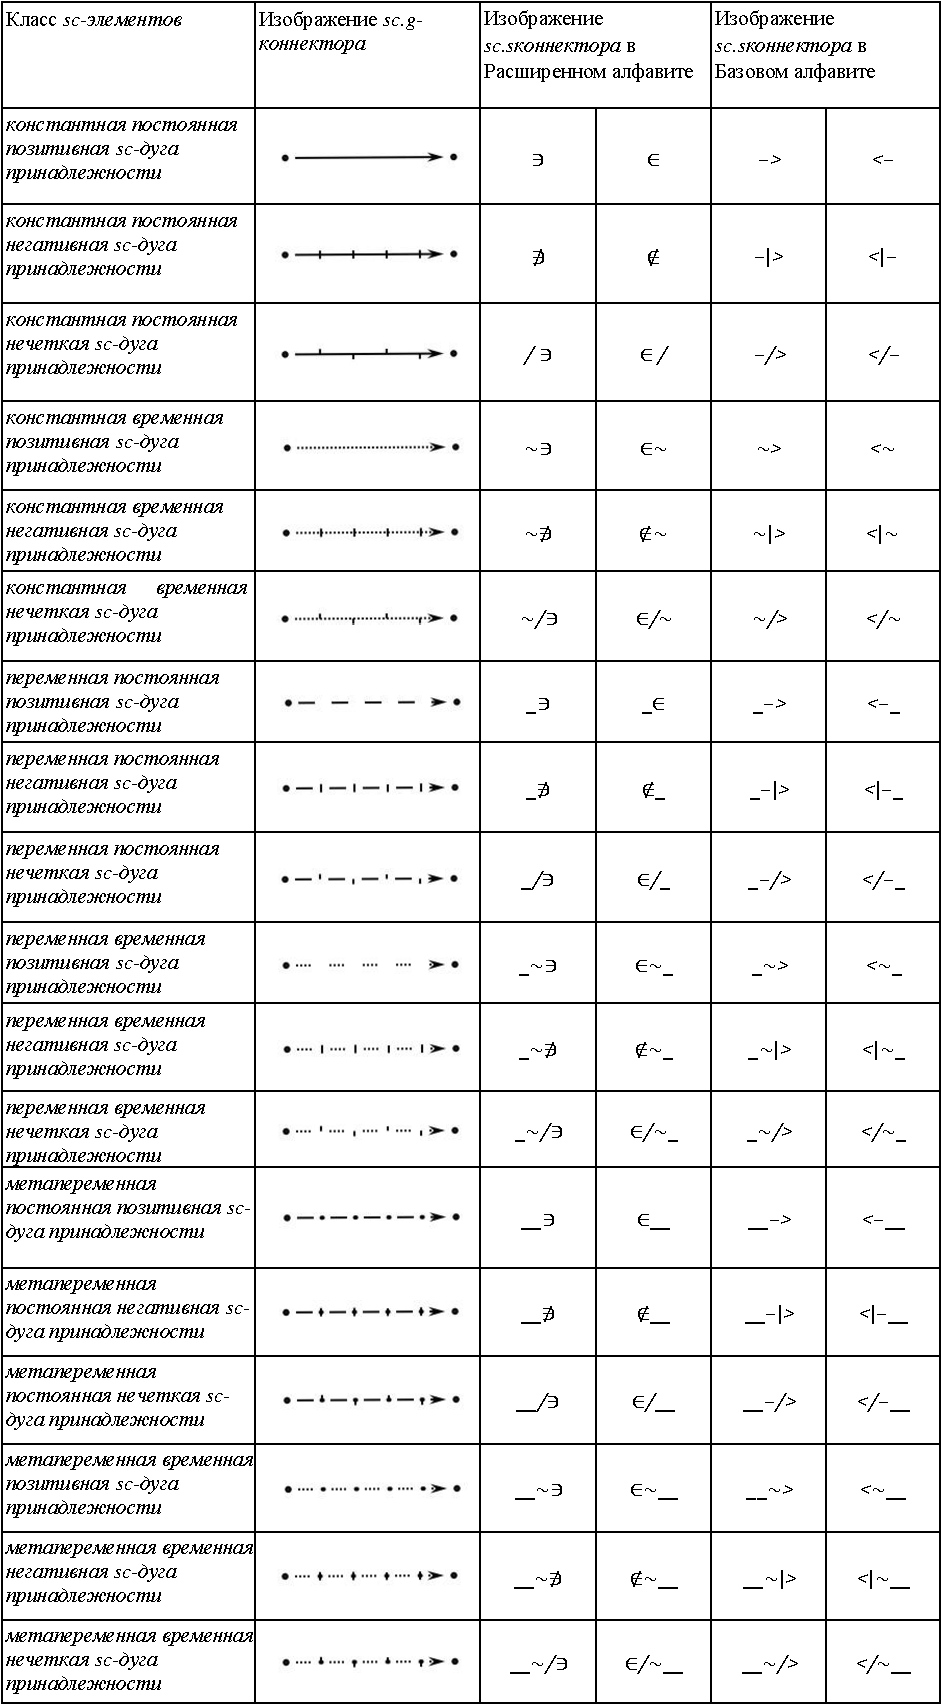
\includegraphics[scale=0.8]{images/intro/scs_membership_connectors.pdf}
	\label{fig:scs_membership_connectors}
\end{figure}


\newpage
\begin{figure}[H]
	\centering
	\caption{Таблица. Алфавит sc.s-коннекторов, соответствующих sc.g-коннекторам, которые не являются sc.g-дугами принадлежности\scnsupergroupsign}
	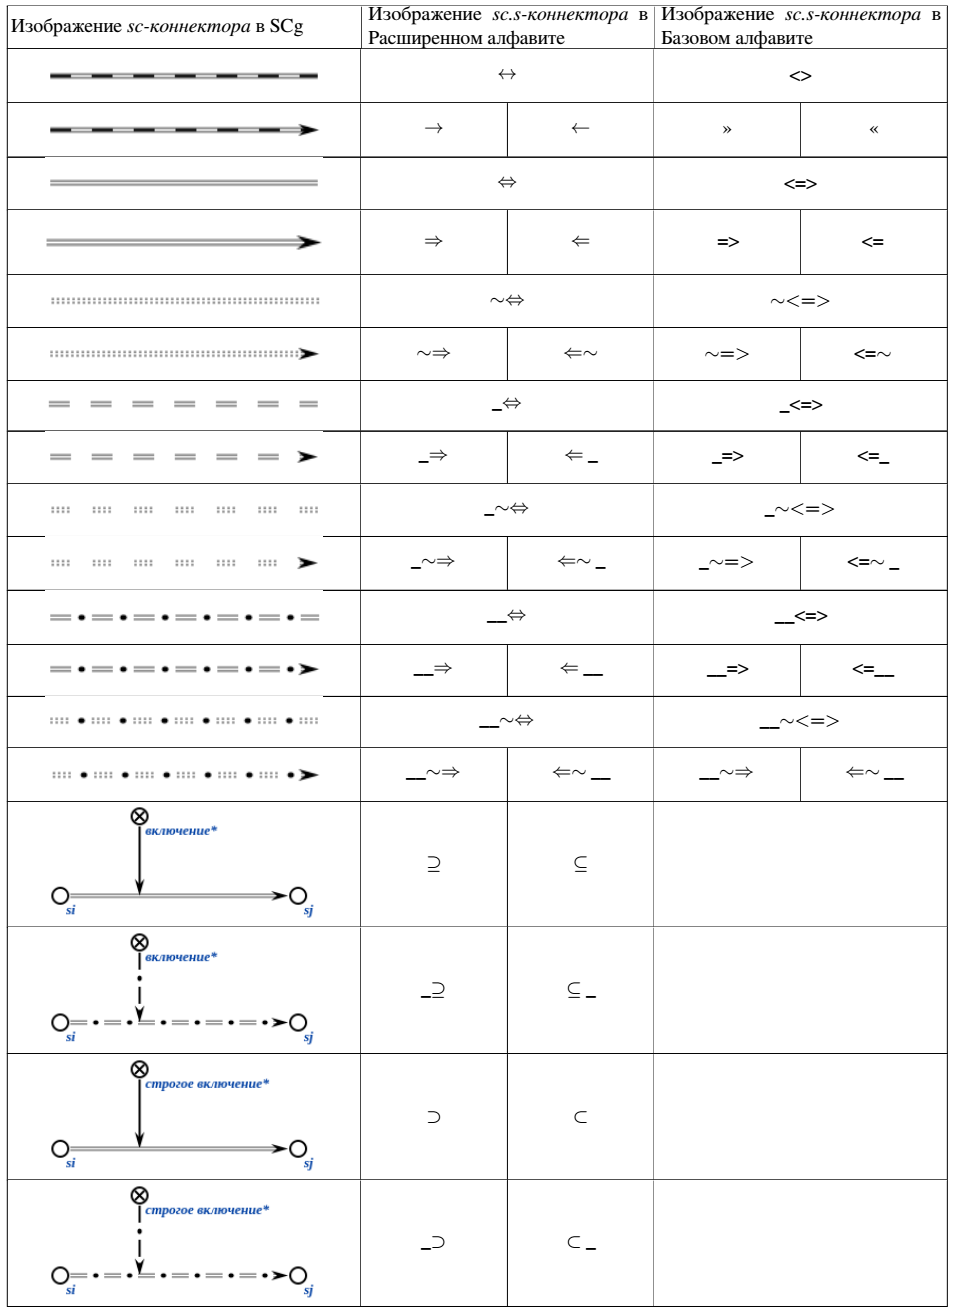
\includegraphics[scale=0.44]{images/intro/scs_non_membership_connectors_1.png}
	\label{fig:scs_non_membership_connectors}
\end{figure}

\newpage

\begin{figure}[H]
	\centering
	\caption{Таблица. Алфавит sc.s-коннекторов, соответствующих sc.g-коннекторам, которые не являются sc.g-дугами принадлежности\scnsupergroupsign (продолжение)}
	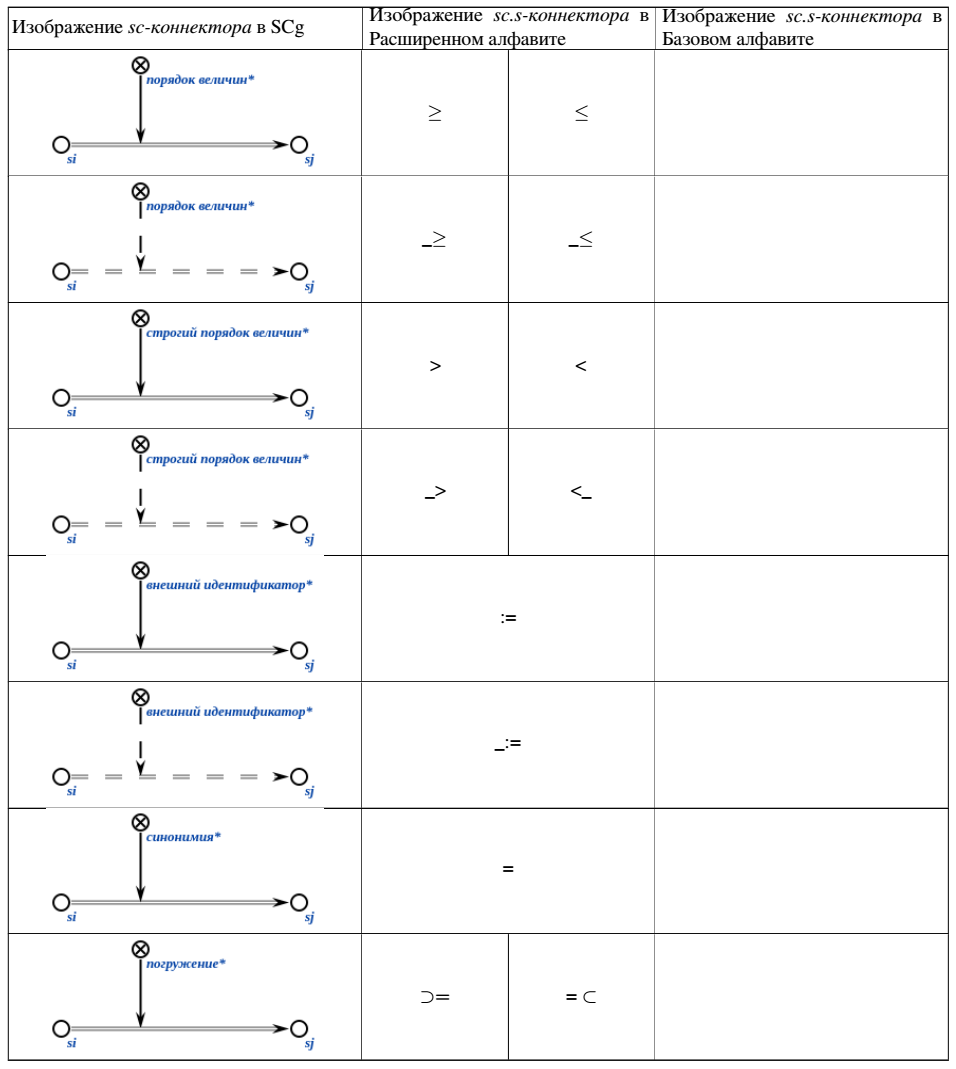
\includegraphics[scale=0.4]{images/intro/scs_non_membership_connectors_2.png}
	\label{fig:scs_non1_membership_connectors}
\end{figure}


Ниже приведены \textit{примеры синтаксической трансформации sc.s-предложений с использованием Расширенного алфавита sc.s-коннекторов и соответствующие семантически эквивалентные конструкции в SCg-коде}.

\bigskip
\begin{SCn}
\scnfilelong{\textbf{\textit{si}}~$\Rightarrow$~\textit{включение*}:~\textbf{\textit{sj}}}
\scnrelfrom{синтаксическая трансформация}{
	\scnfilelong{\textbf{\textit{si}}~$\supseteq$~\textbf{\textit{sj}}}}
\begin{scnindent}
	\scnrelboth{семантическая эквивалентность}{
		\begin{figure}[H]
			\centering
			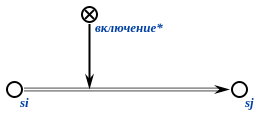
\includegraphics[scale=0.8]{images/intro/scs/sc.s-connectors/examples/scs_transf_inclusion_const.png}
	\end{figure}}
\end{scnindent}
\end{SCn}

\newpage

\begin{figure}[H]
	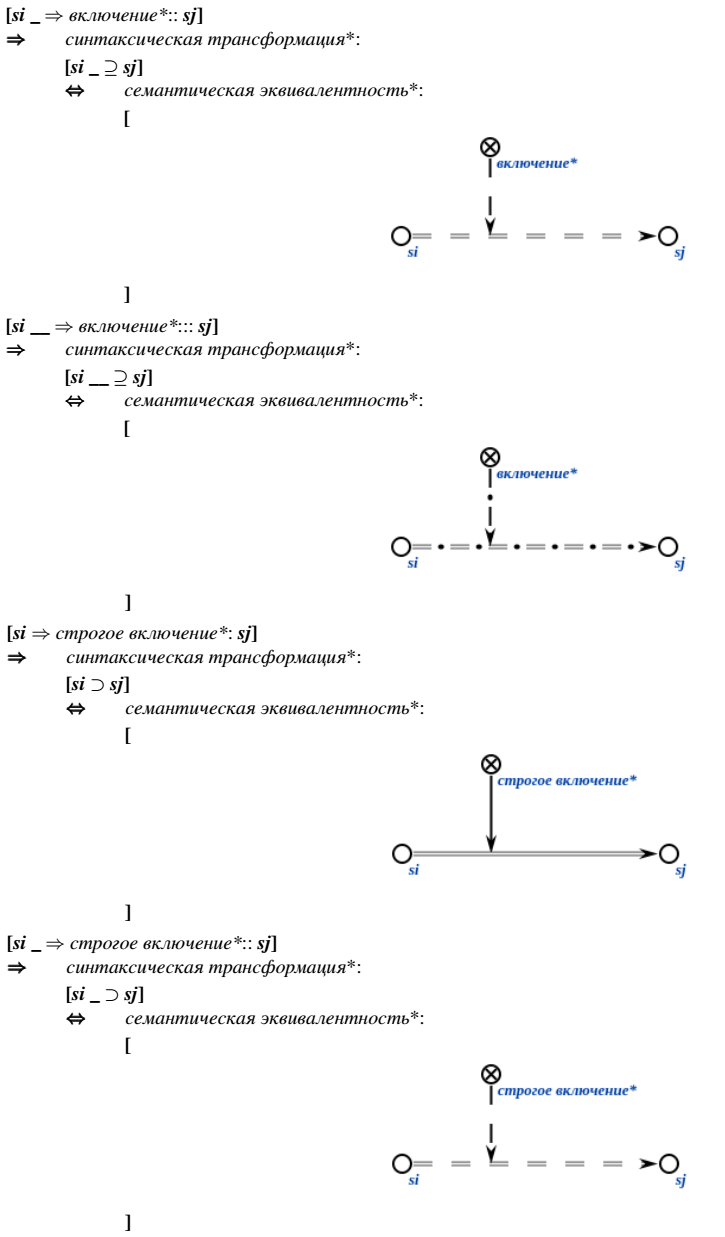
\includegraphics[scale=0.5]{images/intro/scs/sc.s-connectors/examples/example_1.png}
\end{figure}

\newpage
\begin{figure}[H]
	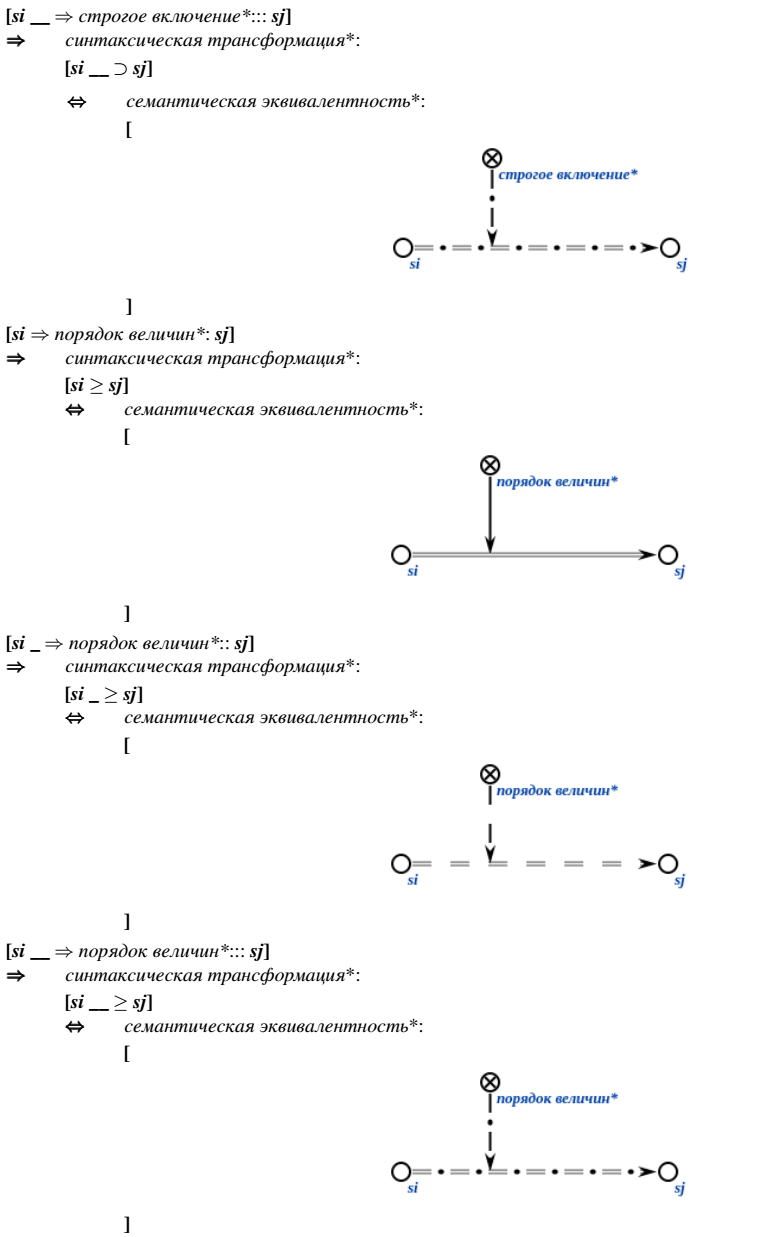
\includegraphics[scale=0.5]{images/intro/scs/sc.s-connectors/examples/example_2.png}
\end{figure}

\newpage
\begin{figure}[H]
	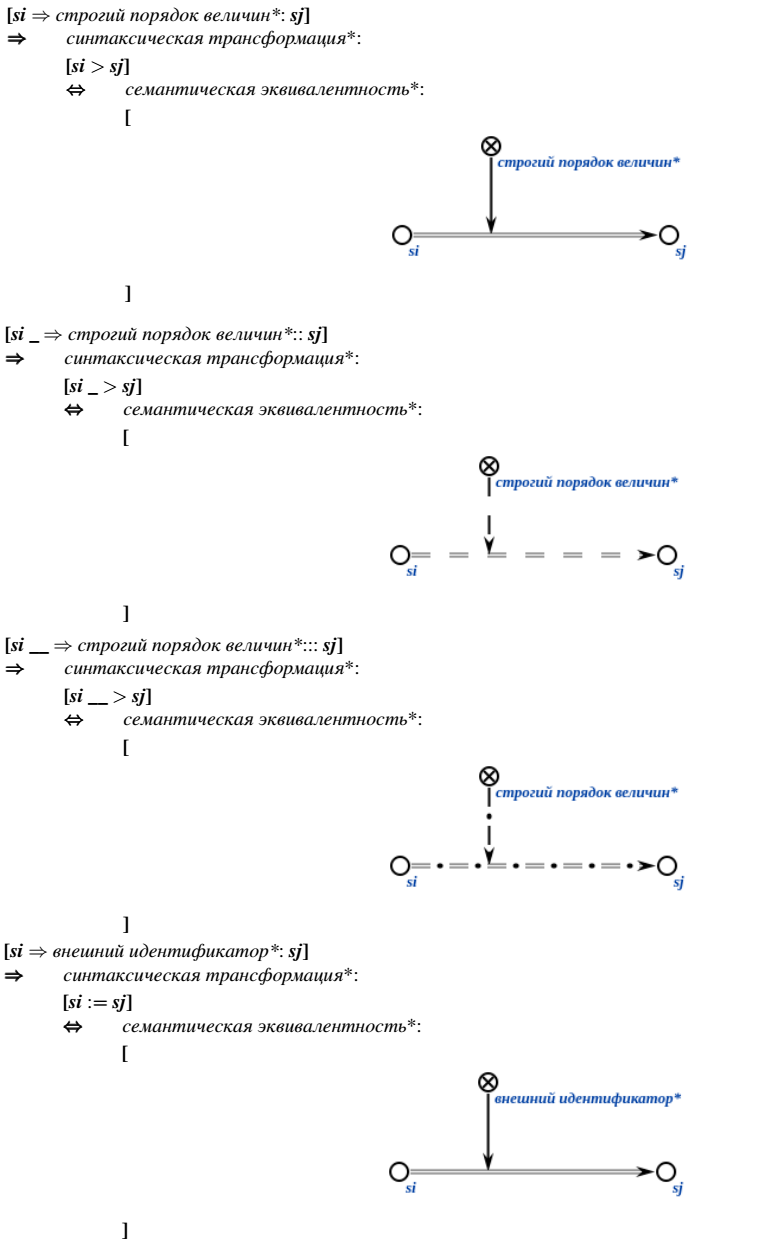
\includegraphics[scale=0.5]{images/intro/scs/sc.s-connectors/examples/example_3.png}
\end{figure}

\newpage
\begin{figure}[H]
	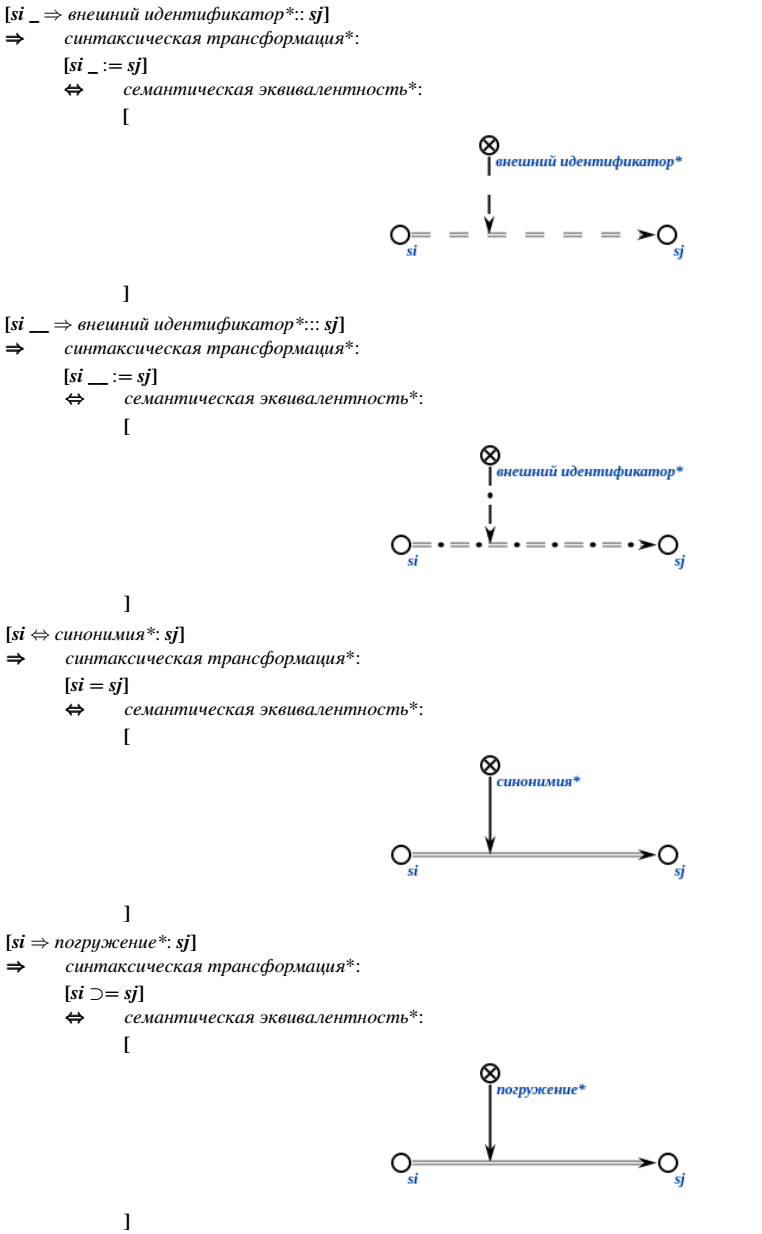
\includegraphics[scale=0.5]{images/intro/scs/sc.s-connectors/examples/example_4.png}
\end{figure}

Аналогичным образом может быть описана трансформация предложений, содержащих любые классы \textit{sc.s-коннекторов}, за исключением тех классов \textit{sc.s-коннекторов}, которые соответствуют классам \textit{sc-коннекторов}, входящим в \textit{Ядро SC-кода}.

В общем случае \textit{sc-элементы}, инцидентные \textit{sc-коннекторам}, классы которых описаны в данном примере, могут быть как \textit{sc-константами}, так и \textit{sc-переменными} (в том числе \textit{sc-метапеременными}). При этом как \textit{переменному sc-коннектору} может соответствовать \textit{константный sc-узел}, так и \textit{константному sc-коннектору} может соответствовать \textit{переменный sc-узел} (например, если возникает необходимость переменному sc-узлу приписать \textit{внешний идентификатор*}). Последняя ситуация встречается не очень часто и возникает в случае, когда область определения соответствующего \textit{отношения} имеет непустое пересечение с классом \textit{sc-переменных}.

\textbf{\textit{Описание примеров выполнения операций, заданных на множестве sc.s-предложений}}

С семантической точки зрения \textit{sc.s-предложение} представляет собой описание некоторого \myuline{маршрута} в соответствующем sc-тексте, который является графовой структурой специального вида и структура которого описывается (изображается) с помощью \textit{sc.s-предложений}. Указанный маршрут "проводится"{} по sc-коннекторам и по связям инцидентности sc-элементов, если маршрут проходит через инцидентные sc-коннекторы. В описании указанного маршрута могут дополнительно указываться множества (чаще всего отношения), которым принадлежат sc-коннекторы, входящие в описываемый маршрут. Кроме того, указанный маршрут в начале и/или в конце может иметь разветвления, когда какой-либо \textit{sc-элемент} \myuline{одинаково} инцидентен нескольким \myuline{однотипным} sc-коннекторам, соединяющим указанный \textit{sc-элемент} с некоторыми другими sc-элементами.

Таким образом каждое указанное разветвление состоит из неограниченного числа ветвей, каждая из которых состоит из одного \textit{sc-коннектора} и одного связываемого им \textit{sc-элемента}.

\subsection{Иерархическое семейство подъязыков, семантически эквивалентных SCs-коду}
\label{sec_scs_extensions}

В рамках \textit{SCs-кода} выделяют \textit{Ядро SCs-кода} и \textit{Направления расширения Ядра SCs-кода}.

\begin{SCn}
\scnheader{Ядро SCs-кода}
\scnidtf{Подъязык \textit{SCs-кода}, который использует минимальный набор синтаксических средств, но при этом имеет семантическую мощность, эквивалентную мощности \textit{SCs-кода} в целом}
\end{SCn}

В \textit{Ядре SCs-кода}:
\begin{textitemize}
	\item используются только \textit{простые sc-идентификаторы}, в том числе \textit{sc-идентификаторы внешних файлов ostis-систем} (sc-выражения не используются);
	\item используются только \textit{sc.s-разделители, изображающие связь инцидентности sc-элементов}, а также sc.s-коннектор, изображающий константную  постоянную позитивную пару принадлежности ("$\in$"{} и "$\ni$"{} в Расширенном алфавите и "{}->{}"{} и "{}<-{}"{} в Базовом алфавите). Другие \textit{sc.s-коннекторы} не используются;
	\item не используются \textit{sc.s-модификаторы} и, соответственно, двоеточия, являющиеся признаком завершения \textit{sc.s-модификаторов};
	\item используются только \textit{простые sc.s-предложения}, которые, как следует из вышеуказанных свойств Ядра SCs-кода, либо состоят из двух \textit{простых sc-идентификаторов}, соединяемых sc.s-коннектором, изображающим константную  постоянную позитивную пару принадлежности, либо трех \textit{простых sc-идентификаторов}, разделенных \textit{sc.s-разделителями, изображающими связь инцидентности sc-элементов}.
\end{textitemize}

Из перечисленных свойств \textit{Ядра SCs-кода} следует, что для представления (изображения) любого \mbox{sc-текста} средствами \textit{Ядра SCs-кода} необходимо для \myuline{всех} (!) sc-элементов этого \mbox{sc-текста} (кроме константных постоянных позитивных пар принадлежности) построить соответствующие им простые \textit{sc-идентификаторы}, то есть необходимо проименовать все указанные sc-элементы. В свою очередь, тип каждого используемого \mbox{sc-элемента} (кроме константных постоянных позитивных пар принадлежности) задается явно путем указания принадлежности этих элементов соответствующим классам sc-элементов, в том числе классам, входящим в \textit{Ядро SC-кода}.

Как видно из приведенного описания, \textit{Ядро SCs-кода} соответствует \textit{Ядру SCg-кода}, за исключением того, что в \textit{Ядре SCg-кода} нет необходимости именовать все изображаемые \textit{sc-элементы}, а также в\textit{ Ядре SCg-кода} присутствуют графические изображения для sc-элементов, принадлежащих соответствующим классам \textit{Ядра SC-кода} и эту принадлежность нет необходимости указывать явно.

Очевидно, что широко практически применять \textit{Ядро SCs-кода} для записи больших фрагментов баз знаний неудобно и неэффективно. Тем не менее, с практической точки зрения \textit{Ядро SCs-кода} может использоваться, например, для обмена информацией со сторонними средствами представления графовых конструкций, рассчитанными на представление информации в виде триплетов (например, RDF-хранилищ).
Для обеспечения возможности более широкого практического использования необходимы синтаксические расширения \textit{Ядра SCs-кода} в целях:
\begin{textitemize}
	\item минимизации числа идентифицируемых (именуемых) sc-элементов путем использования \textit{sc-выражений} и ликвидации необходимости идентифицировать (именовать) \myuline{все} (!) \textit{sc-элементы};
	\item сокращения текста путем минимизации числа повторений одного и того же \textit{sc-идентификатора} путем соединения \textit{sc.s-предложений};
	\item повышение уровня наглядности, "читабельности"{} \textit{sc.s-текстов}.
\end{textitemize}

\begin{SCn}
\scnheader{Первое направление расширения Ядра SCs-кода}
\scnidtf{Первое направление расширения Ядра SCs-кода \myuline{и всех иных его расширений}}
\end{SCn}

По сравнению с \textit{Ядром SCs-кода} в \textit{Первом направлении расширения Ядра SCs-кода} вместо \textit{sc-идентификато|-ров}, являющихся идентификаторами (именами), которые взаимно однозначно соответствуют синонимичным им (представляемым ими) sc-коннекторам, вводятся \textit{sc.s-коннекторы}, каждый из которых соответствует не одному конкретному \textit{sc-коннектору}, а некоторому классу однотипных sc-коннекторов. Очевидно, что это ликвидирует необходимость \myuline{каждому} sc-коннектору приписывать уникальный \textit{sc-идентификатор}. Кроме того, \textit{Алфавит sc.s-коннекторов\scnsupergroupsign} включает в себя элементы этого Алфавита (классы \myuline{синтаксически} эквивалентных \textit{sc.s-коннекторов}), которые соответствуют \myuline{всем} (!) элементам \textit{Алфавита sc-коннекторов\scnsupergroupsign}, но при этом дополнительно включают в себя и другие элементы \textit{Алфавита sc.s-коннекторов\scnsupergroupsign}, которые соответствуют часто используемым \myuline{семантически} явно выделяемым классам sc-коннекторов. К таким дополнительно вводимым классам \textit{sc.s-коннекторов} относятся \textit{константные sc.s-коннекторы} включения множеств ("$\supset$"{} или "$\subset$"{}), \textit{переменные sc.s-коннекторы} включения множеств ("$\_\supset$"{} или "$\subset\_$"{}), \textit{sc.s-коннектор} синонимии ("$=$"{}), \textit{sc.s-коннектор} погружения ("$=\subset$"{} или "$\supset=$"{}) и другие.

Заметим, что указанное расширение \textit{Алфавита SCs-кода\scnsupergroupsign} \textit{sc.s-коннекторов} аналогично расширенному \textit{Алфавиту sc.g-коннекторов} в \textit{SCg-коде} и ликвидирует необходимость (как и в \textit{SCs-коде}) явно специфицировать (средствами \textit{SCs-кода}) синтаксически выделяемые классы \textit{sc.s-коннекторов}.

\textbf{\textit{Второе направление расширения Ядра SCs-кода}}

Во \textit{Втором направлении расширения Ядра SCs-кода} вводятся модификаторы \textit{sc.s-коннекторов} (\textit{\mbox{sc.s-модификаторы}}), которые позволяют достаточно компактно дополнительно специфицировать \mbox{sc-коннекторы}, изображаемые (представляемые) соответствующими \textit{sc.s-коннекторами}. Речь идет о такой часто востребованной форме спецификации sc-коннекторов, как указание множества (возможно, нескольких множеств), которому принадлежит специфицируемый  sc-коннектор (чаще всего, таким множеством является \textit{бинарное отношение} (в частности, \textit{ролевое отношение}) или \textit{квазибинарное отношение}).

\begin{SCn}
\scnheader{sc.s-модификатор*}
\scniselement{отношение}
\begin{scnindent}
	\scnidtf{относительное понятие}
\end{scnindent}	
\scnidtf{модификатор sc.s-коннектора*}
\textit{sc-идентификатор}, который (1) находится либо между \textit{sc.s-коннектором} и \textit{двоеточием}, либо между \textit{двоеточиями} и (2) обозначает множество (чаще всего, отношение), которому принадлежит sc-коннектор, изображаемый ближайшим предшествующим \textit{sc.s-коннектором}. Два подряд идущих двоеточия ("::"{}) обозначают, что указанное множество связано с указанным sc-коннектором \textit{\myuline{переменной} позитивной постоянной sc-дугой принадлежности}.
\end{SCn}

Очевидно, что, если не использовать \textit{sc.s-модификаторы}, указанного вида спецификация \textit{sc-коннекторов} средствами \textit{SCs-кода} будет выглядеть значительно более громоздкой.

\textbf{\textit{Третье направление расширения Ядра SCs-кода}}

В \textit{Третьем направлении расширения Ядра SCs-кода} осуществляется переход от использования только \textit{простых sc-идентификаторов} к использованию как \textit{простых sc-идентификаторов}, так и \textit{sc-выражений}, а также к использованию \textit{sc.s-представлений некоторых неидентифицируемых sc-узлов}. Это существенно сокращает число придумываемых \textit{простых sc-идентификаторов}, так как каждое \textit{sc-выражение} в конечном счете — это комбинация \textit{простых sc-идентификаторов}, построенная по правилам, которые достаточно легко семантически интерпретируются. Если проводить аналогию с SCg-кодом, то очевидно, что \textit{\mbox{sc-выражение}}, ограничиваемое фигурными скобками, есть не что иное, как информационная конструкция, ограничиваемая \textit{sc.g-контуром}, а \textit{sc-выражение}, ограничиваемое квадратными скобками есть не что иное, как информационная конструкция, ограничиваемая \textit{sc.g-рамкой}. Отличие здесь заключается в том, что круглыми и квадратными скобками можно ограничивать только линейные информационные конструкции (цепочки символов).

\begin{SCn}
\scnheader{sc.s-представление неидентифицируемого sc-узла}
\scnidtf{изображение (представление) неидентифицируемого (неименуемого) sc-узла в sc.s-тексте}
\scnidtf{sc.s-обозначение неименуемой сущности, не являющейся парой, обозначаемой sc-коннектором}
\scnidtf{sc.s-представление sc-узла, не являющееся sc-идентификатором (именем этого sc-узла)}
\end{SCn}

Если одно и то же обозначение неименуемой сущности встречается в \myuline{разных} \textit{sc.s-предложениях}, то считается, что это обозначения \myuline{разных} сущностей, то есть изображения \myuline{разных} sc-узлов.

\textbf{\textit{Четвертое направление расширения Ядра SCs-кода}}

В \textit{Четвертом направлении расширения Ядра SCs-кода} осуществляется переход от использования только \textit{простых sc.s-предложений} к использованию также \textit{sc.s-предложений}, построенных с помощью \textit{\mbox{Операции} присоединения sc.s-предложения*}. В результате этого, благодаря "склеиванию"{} одинаковых \textit{\mbox{sc-идентификаторов}}, а также "склеиванию"{} синтаксически эквивалентных \textit{\mbox{sc.s-коннекторов}} с одинаковыми \textit{\mbox{sc.s-модификаторами}} (несмотря на то, что эти "склеиваемые"{} \textit{sc.s-коннекторы} соответствуют \myuline{разным} \mbox{sc-коннекторам}), существенно сокращается число копий используемых \textit{\mbox{sc-идентификаторов}} и \textit{\mbox{sc.s-коннекторов}} с их \textit{\mbox{sc.s-модификаторами}}.

\textbf{\textit{Пятое направление расширения Ядра SCs-кода}}

В \textit{Пятом направлении расширения Ядра SCs-кода} разрешается использование \textit{присоединенных \mbox{sc.s-предложений}}. В результате этого \textit{sc.s-тексты} становятся более компактными и удобными для восприятия за счет снижения числа дублируемых \textit{sc-идентификаторов} и более широких возможностей их структуризации.

\section{Язык внешнего форматированного представления конструкций SC-кода --- SCn-код (Semantic Code natural)}
\markboth{Язык внешнего форматированного представления конструкций SC-кода --- SCn-код}{Язык внешнего форматированного представления конструкций SC-кода --- SCn-код}
\label{sec_scn}

\begin{SCn}
\begin{scnrelfromlist}{подраздел}
	\scnitem{\ref{sec_scn_syntax}~\nameref{sec_scn_syntax}}
	\scnitem{\ref{sec_scn_semantics}~\nameref{sec_scn_semantics}}
	\scnitem{\ref{subsec_latex}~\nameref{subsec_latex}}
\end{scnrelfromlist}

\bigskip

\begin{scnrelfromlist}{ключевой знак}
	\scnitem{SCn-код}
	\scnitem{Алфавит SCn-кода\scnsupergroupsign}
	\scnitem{Синтаксис SCn-кода}
	\scnitem{Денотационная семантика SCn-кода}
\end{scnrelfromlist}

\begin{scnrelfromlist}{ключевое понятие}
	\scnitem{страница sc.n-текста}
	\scnitem{строка sc.n-текста}
	\scnitem{линия разметки sc.n-текста}
	\scnitem{sc.n-предложение}
	\scnitem{sc.n-элемент}
	\scnitem{sc.n-коннектор}
	\scnitem{sc.n-ребро}
	\scnitem{sc.n-дуга}
	\scnitem{sc.n-контур}
	\scnitem{sc.n-рамка}
\end{scnrelfromlist}
\end{SCn}

\subsection*{Введение в \ref{sec_scn}}

\begin{SCn}
\scnheader{SCn-код}
\scnidtf{Язык структурированного представления знаний \textit{ostis-систем}}
\scnidtf{Язык внешнего форматированного представления конструкций внутреннего языка \textit{ostis-систем}}
\end{SCn}

\textbf{\textit{SCn-код}} является языком структурированного внешнего представления текстов \textit{SC-кода} и представляет собой синтаксическое расширение \textit{SCs-кода}, направленное на повышение наглядности и компактности текстов \textit{SCs-кода}. 

\textit{SCn-код} позволяет перейти от линейных текстов \myuline{SCs-кода} к форматированным и фактически двухмерным текстам, в которых появляется декомпозиция исходного линейного текста \myuline{SCs-кода} на \myuline{строчки}, размещенные \scnqqi{по вертикали}. При этом начало всех \myuline{строчек} текста фиксировано и определяется известным и ограниченным набором правил, что дает возможность использовать это при форматировании \myuline{sc.n-текста} (текста, принадлежащего \textit{SCn-коду}, см. \scncite{Standart2021}).

\subsection{Синтаксис SCn-кода}
\label{sec_scn_syntax}

\textit{Алфавит SCs-кода\scnsupergroupsign} является также алфавитом символов и \textit{SCn-кода}, то есть \textit{алфавиты}* этих языков совпадают.

\textit{SCn-код} --- язык, каждый \textit{текст} которого задается:
\begin{textitemize}
	\item множеством входящих в него \textit{символов};
	\item отношением порядка (последовательности) \textit{символов} по "горизонтали"{};
	\item отношением порядка(последовательности) \textit{символов} по "вертикали"{}.
\end{textitemize}

\begin{SCn}
	\scnheader{sc.n-текст}
	\scnidtf{текст \textit{SCn-кода}}
	\scnidtf{последовательность предложений \textit{SCn-кода}}
	\scnidtf{последовательность предложений \textit{SCn-кода}, каждое из которых не является частью какого-либо другого предложения из \myuline{этой} последовательности}
\end{SCn}

Важной особенностью \textit{SCn-кода} является \scnqqi{двухмерный} характер его текстов. Это проявляется в том, что для каждого фрагмента текста \textit{SCn-кода} важное значение имеет величина отступа от левого края \textit{строчки}.

Символ, входящий в состав \textit{двухмерного текста}, в общем случае может иметь четыре "соседних"{} \textit{символа}: 
\begin{textitemize}
	\item \textit{символ}, находящийся от него \myuline{слева} в рамках той же \textit{строчки};
	\item \textit{символ}, находящийся от него \myuline{справа} в рамках этой же \textit{строчки};
	\item \textit{символ}, находящийся строго \myuline{над} ним в предыдущей \textit{строчке};
	\item \textit{символ}, находящийся строго \myuline{под ним} в следующей \textit{строчке} текста.
\end{textitemize}

Благодаря тому, что в состав \textit{sc.n-текстов} могут входить и \textit{sc.s-тексты}, и \textit{sc.g-тексты} (ограниченные \textit{sc.n-контуром}), \textit{SCn-код} можно считать интегратором различных внешних языков представления знаний.  Это дает возможность при визуализации и разработке базы знаний ostis-системы недостатки одного из предлагаемых вариантов внешнего представления sc-текстов (\textit{SCg-кода}, \textit{SCs-кода}, \textit{SCn-кода}) компенсировать достоинствами других вариантов.

\begin{SCn}
\scnheader{страница sc.n-текста}
\scnidtf{страница, на которой размещается sc.n-текст}
\end{SCn}

Если \textit{sc.n-текст} является частью какого-либо другого файла, разделяемого на страницы, например, публикации какой-либо части базы знаний, то \textit{sc.n-страницей} считается только часть страницы, на которой изображен \textit{sc.n-текст}, в то время как страница указанного файла может быть больше за счет, например, белых полей по краям страницы, необходимых для последующей распечатки.

\textbf{\textit{строчка sc.n-текста}}

Максимальное количество символов в строчках \textit{sc.n-текста} для каждого \textit{sc.n-текста} фиксировано и определяется конкретным вариантом размещения \textit{sc.n-текста}. При этом, в зависимости от отступов в рамках конкретного \textit{sc.n-предложения}, строчка \textit{sc.n-текста} может начинаться не с левого края \textit{sc.n-текста} (но всегда с какой-то из вертикальных линий разметки) и иметь произвольную длину, ограничиваемую правой границей \textit{sc.n-страницы}.

\begin{SCn}
\scnheader{линия разметки sc.n-текста}
\scnidtf{табуляционная линия sc.n-текста}
\scnidtf{вертикальная линия разметки sc.n-текста}
\scnidtf{вертикальная табуляционная линия}
\scnidtf{вертикальная линия, используемая для упрощения восприятия sc.n-текстов и показывающая уровень отступа для компонентов sc.n-предложений}
\end{SCn}

1-я линия разметки ограничивает левый край \textit{sc.n-страницы}, 2-я линия разметки располагается примерно между 5 и 6 символами строчки и так далее. Расстояние между линиями разметки может меняться в зависимости от размера шрифта, однако в рамках одного \textit{sc.n-текста} всегда остается одинаковым. Общее количество линий разметки ограничивается максимально возможной шириной \textit{sc.n-страницы} в конкретном файле \textit{ostis-системы}, содержащем данный \textit{sc.n-текст}.

\begin{SCn}
\scnheader{следует отличать*}
\begin{scnhaselementset}
	\scnitem{страница sc.n-текста}
	\scnitem{строчка sc.n-текста}
	\scnitem{строка}	
\end{scnhaselementset}
\end{SCn}

Все компоненты \textit{sc.s-текстов} используются также и в \textit{sc.n-текстах}:
\begin{textitemize}
	\item \textit{sc-идентификаторы};
	\item \textit{sc.s-коннекторы};
	\item модификаторы \textit{sc.s-коннекторов} с соответствующими разделителями (двоеточиями)
	\item разделители, используемые в sc-выражениях, обозначающих sc-множества, заданные перечислением элементов с соответствующими разделителями (\textit{точкой с запятой} или \textit{круглым маркером});
	\item \textit{круглые маркеры} в перечислениях идентификаторов \mbox{sc-элементов}, связанных однотипными sc-коннекторами с однотипными модификаторами с заданным sc-элементом;
	\item разделители предложений (двойные точки с запятой) (опускаются при преобразовании \mbox{sc.s-предложений} в \mbox{sc.n-предложения});
	\item ограничители присоединенных \textit{sc.s-предложений} (опускаются при преобразовании sc.s-предложений в sc.n-предложения).
\end{textitemize}

В отличие от \textit{sc.s-текстов} в \textit{sc.n-текстах}:
\begin{textitemize}
	\item добавляются новые виды \textit{sc-выражений} (а именно --- sc-выражений, имеющих двухмерный характер);
	\item добавляется новый вид разделителей предложений --- пустая строчка;
	\item меняется размещение предложений с учетом двухмерного характера такого размещения.
\end{textitemize}

В \textit{SCn-коде} по сравнению с \textit{SCs-кодом} добавляются новые виды \textit{sc-выражений}:
\begin{textitemize}
	\item \textit{sc-выражение}, представляющее собой двухмерный \textit{\mbox{sc.n-текст}}, ограниченный \textit{sc.n-контуром} или \textit{sc.n-рамкой}. Каждый \textit{sc.n-контур} изображается условно в виде \textit{открывающей фигурной скобки} и расположенной строго \myuline{под} ней через несколько строчек \textit{закрывающей фигурной скобки}. Внутри указанных скобок (начиная от линии вертикальной разметки, на которой расположены сами скобки, и до правого края \textit{страницы}) размещается sc.n-текст. Полученный sc.n-контур является изображением структуры, являющейся результатом трансляции указанного sc.n-текста в SC-код. Каждая \textit{sc.n-рамка} изображается аналогичным образом, только вместо \textit{фигурных скобок} в ней используются \textit{квадратные скобки}, либо \textit{квадратные скобки} с \textit{восклицательным знаком} (в случае файла-образца);
	\item \textit{sc-выражение}, представляющее собой двухмерный \textit{sc.g-текст}, ограниченный \textit{\mbox{sc.n-контуром}} или \textit{\mbox{sc.n-рамкой}}.
	\item \textit{sc-выражение}, представляющее собой ограниченное \textit{sc.n-рамкой} двухмерное графическое изображение \textit{информационной конструкции}, закодированной в некотором \textit{файле ostis-системы}. Такой \textit{информационной конструкцией} может быть таблица, рисунок, фотография, диаграмма, график и многое другое.
\end{textitemize}

Нетрудно заметить, что \textit{sc.n-контур} является, по сути, двухмерным эквивалентом \textit{sc-выражения структуры}, а \textit{sc.n-рамка} --- двухмерным эквивалентом \textit{sc-выражения внутреннего файла \mbox{ostis-системы}} или \textit{sc-выражения, обозначающего файл-образец ostis-системы}.

\begin{SCn}
\scnheader{sc.n-рамка}
\scnidtf{ограничитель изображения файла \myuline{ostis-системы}, используемый в \myuline{sc.n-предложениях}}
\end{SCn}

Обозначается с помощью квадратных скобок: \scnqqi{ [ }, \scnqqi{ ] }.

С формальной точки зрения \textit{sc.n-рамка} всегда представляет собой \myuline{одну} \textit{строчку sc.n-текста}. Это означает, что \textit{sc.n-рамка} не может быть синтаксически разделена на части в рамках того \textit{sc.n-текста}, в котором она используется, и внутрь нее не могут вставляться, например, \textit{присоединенные sc.n-предложения} или какой-либо другой текст (за исключением случаев, когда \textit{sc.n-рамка} содержит \textit{sc.n-текст}, но в этом случае указанный \textit{sc.n-текст} все равно будет рассматриваться как целостный внешний файл, а не как фрагмент окружающего его \textit{sc.n-текста}). 

\begin{SCn}
	\scnheader{sc.n-контур}
	\scnidtf{используемый в sc.n-предложениях ограничитель, являющийся изображением структуры}
\end{SCn}

Обозначается с помощью фигурных скобок: \scnqqi{ \textbraceleft }, \scnqqi{ \textbraceright } .

Понятие \textbf{\textit{sc.n-предложения}} является естественным обобщением понятия \textit{sc.s-предложения}. Более того, аналогичным для \textit{sc.s-предложений} образом вводятся понятия:
\begin{textitemize}
	\item \textit{простого sc.n-предложения}
	\item \textit{сложного sc.n-предложения}
	\item \textit{sc.n-предложения, содержащего присоединенные sc.n-предложения}
	\item \textit{sc.n-предложения, не содержащего присоединенные sc.n-предложения}
	\item \textit{присоединенного sc.n-предложения}
	\item \textit{неприсоединенного sc.n-предложения}
\end{textitemize}

\myuline{Если} каждое \textit{неприсоединенное sc.s-предложение} \myuline{либо} являетcя первым предложением \textit{sc.s-текста}, \myuline{либо} начинается после \textit{разделителя sc.s-предложений} (\textit{двойной точки с запятой}), \myuline{то} каждое \textit{неприсоединенное sc.n-предложение} начинается с начала новой строчки.

\myuline{Если} каждое \textit{присоединенное sc.s-предложение} начинается либо после открывающего ограничителя присоединенных sc.s-предложений (открывающей круглой скобки со звездочкой), \myuline{либо} после \textit{разделителя sc.s-предложений}, \myuline{то} каждое \textit{присоединенное sc.n-предложение} начинается с новой строчки под sc-идентификатором, которым завершается то sc.n-предложение (и соответственно, sc.s-предложение), в которое встраивается данное \textit{присоединенное sc.n-предложение}.

Первый \textit{sc-идентификатор}, входящий в состав \textit{sc.n-предложения} до \textit{sc.s-коннектора} выделяется \myuline{жирным} курсивом;
В \textit{sc.n-предложениях двойная точка с запятой} не используется в качестве признака завершения этих предложений и, соответственно, не используется в качестве разделителя \textit{sc.n-предложений}. Таким разделителем является \textit{пустая строчка}.

Благодаря двухмерности \textit{SCn-кода} появляются более широкие возможности (степени свободы) для наглядного и компактного размещения \textit{sc.n-предложений}.

При оформлении \textit{sc.n-предложения} осуществляется четкая \myuline{табуляция} всех присоединенных к нему \textit{sc.n-предложений}, присоединяемых к исходному "по вертикали"{}. Вертикальная линия табуляции задает левую границу исходного (максимального) sc.n-предложения или левую границу присоединенного \textit{sc.n-предложения}, присоединяемого "по вертикали". Левая граница sc.n-предложения задает начало первого sc-идентификатора, входящего в состав этого \mbox{sc.n-предложения}, а также начало \textit{sc.s-коннектора}, инцидентного указанному \mbox{sc-идентификатору} и размещаемого \myuline{строго под} этим \textit{sc-идентификатором}. Расстояние между вертикальными табуляционными линиями фиксировано и примерно равно максимальной длине \textit{sc.s-коннектора}.

\subsection{Денотационная семантика SCn-кода}
\label{sec_scn_semantics}

\textit{SCn-код} предназначен для представления \textit{sc-графов} в виде отформатированных по заданным правилам последовательностей символов, в которых также могут быть использованы базовые средства гипермедиа, такие как графические изображения, а также средства навигации между частями sc.n-текстов. \textit{SCn-код} имеет много общего с \textit{SCs-кодом} и, за исключением некоторых особенностей, является его двумерным форматированным вариантом.

Поскольку по отношению к \textit{SCn-коду} \textit{SCs-код} является \textit{синтаксическим ядром языка*}, \textit{SCn-код} можно рассматривать как результат интеграции нескольких направлений расширения \textit{SCs-кода}, в основе которых лежат правила синтаксической трансформации \textit{sc.s-текстов} и \textit{sc.n-текстов}, ориентированные на повышение эффективности использования тех возможностей обеспечения наглядности и компактности \textit{sc.n-текстов}, которые открываются при переходе от линейности \textit{sc.s-текстов} к двухмерности \textit{sc.g-текстов}.

Каждый \textit{sc.n-текст} может быть представлен в нескольких вариантах идентификации \textit{sc-элементов} представляемого \textit{sc-графа}:
\begin{textitemize}
	\item с использованием \textit{системных идентификаторов}, которые носят интернациональный характер;
	\item с использованием \textit{основных идентификаторов*} для русскоязычных пользователей;
	\item с использованием \textit{основных идентификаторов*} для англоязычных пользователей.
\end{textitemize}

Каждый \textit{sc.n-текст} представляет собой последовательность \textit{sc.n-статей} (аналог форматированного естественно-языкового текста). Каждая \textit{sc.n-статья}, в свою очередь, представляет собой последовательность \textit{sc.n-предложений}, в начале которой помещается заголовок \textit{sc.n-статьи}, который представляет собой идентификатор ключевого \textit{sc-элемента} того \textit{sc-графа}, который представляется данной \textit{sc.n-статьей}. С семантической точки зрения указанный \textit{sc-граф} является семантической окрестностью, центром которой является указанный ключевой sc-элемент. При этом ключевой sc-элемент некоторой статьи обязательно входит в состав каждого из \textit{sc.n-предложений}, но необязательно является компонентом ключевого (самого первого, считая от начала предложения) \textit{sc-коннектора} данного \textit{sc.n-предложения}. Входящие в \textit{sc.n-статью} \textit{sc.n-предложения} являются \textit{sc.s-предложениями} либо некоторыми их модификациями(см. \scncite{IMS})

Разделителями \textit{sc.n-предложений} (как и \textit{sc.s-предложений}) являются двойные точки с запятой. Этот же разделитель отделяет заголовок \textit{sc.n-статьи} от первого предложения этой \textit{sc.n-статьи}. При этом заголовок \textit{sc.n-статьи} можно трактовать как вырожденное \textit{sc.n-предложение}, состоящее только из одного идентификатора.

В отличие от \textit{sc.s-текстов}: в \textit{sc.n-текстах} \textit{sc.s-коннектор} может быть инцидентен предшествующему \textit{sc-идентификатору} (как простому, так и \textit{sc-выражению}) не только \scnqqi{по горизонтали}, но и \scnqqi{по вертикали}. Для этого \textit{sc.s-коннектор} размещается строго \myuline{под} предшествующим ему sc-идентификатором.

Кроме того \scnqqi{по вертикали} \textit{sc-идентификатор} может быть инцидентен не одному, а \myuline{нескольким} \textit{sc.s-коннекторам}, которые последовательно \scnqqi{по вертикали} размещаются \myuline{под} указанным \textit{sc-идентификатором}. Это позволяет в рамках одного \textit{sc.n-предложения} представлять произвольное число \scnqqi{ответвлений} от каждого sc-идентификатора, то есть произвольное число \textit{sc.s-коннекторов}, инцидентных этому \textit{sc-идентификатору}.
Каждый \textit{sc-идентификатор}, включая \textit{sc-выражение}, ограничиваемого фигурными или квадратными скобками, должен размещаться сразу правее вертикальной разметочной линии, если \myuline{под ним} размещается \textit{sc.s-коннектор}.

Каждый \textit{sc.s-коннектор} выделяется жирным некурсивным шрифтом и, если он находится \myuline{под} инцидентным ему \textit{sc-идентификатором}, размещается строго между двумя вертикальными разметочными линиями, прижимаясь при этом к левой из этих двух разметочных линий.

Поскольку по отношению к \textit{SCn-коду} \textit{SCs-код} является \textit{синтаксическим ядром языка*}, \textit{SCn-код} можно рассматривать как результат интеграции нескольких направлений расширения \textit{SCs-кода}, в основе которых лежат правила синтаксической трансформации \textit{sc.s-текстов} и \textit{sc.n-текстов}, ориентированные на повышение эффективности использования тех возможностей обеспечения наглядности и компактности \textit{sc.n-текстов}, которые открываются при переходе от линейности \textit{sc.s-текстов} к двухмерности \textit{sc.g-текстов}.

Рассмотрим фрагмент \textit{sc.g-текста}, изображенного на \textit{\nameref{scg_example_scs}}.
На данном фрагменте представлен класс материальных объектов, включающий: Землю, Луну, Солнце, Марс. Материальный объект "Луна" имеет два основных идентификатора на русском и английском языках. "Земля" и "Марс" связаны с "Солнце" с помощью отношения "вращаться вокруг*". "Луна" связана с "Земля" с помощью отношения "спутник*"(см. \scncite{Zhmyrko2022}).

\begin{figure}
	\centering
	\caption{Рисунок. Фрагмент sc.g-текста}
	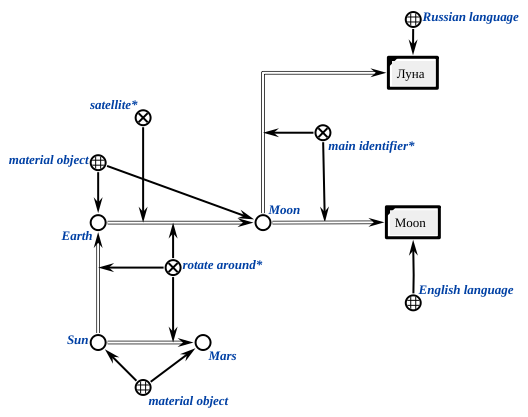
\includegraphics[scale=0.8]{images/intro/scs/example_transf_scg.png}
	\label{scg_example_scs}
\end{figure}

Любой \textit{sc.g-текст} можно легко представить с помощью \textit{sc.s-текста}. Соответственно, описанный выше фрагмент \textit{sc.g-текста} представлен в \textit{sc.s-тексте} на \textit{\nameref{scg_example_scs1}}.

\begin{figure}
	\centering
	\caption{Рисунок. Фрагмент sc.s-текста, соответствующий sc.g-тексту}
	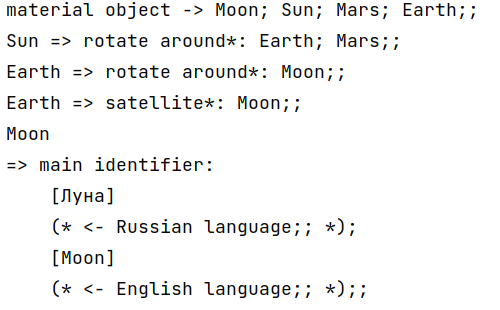
\includegraphics[width=0.5\textwidth]{images/intro/scs/example_transf_scs.png}
	\label{scg_example_scs1}
\end{figure}

На \textit{\nameref{scs_example_scn}} продемонстрирован фрагмент вышеуказанного текста в \textit{SCn-коде}.

\begin{figure}
	\centering
	\caption{Рисунок. Фрагмент sc.n-текста, соответствующий sc.s/sc.g-тексту}
	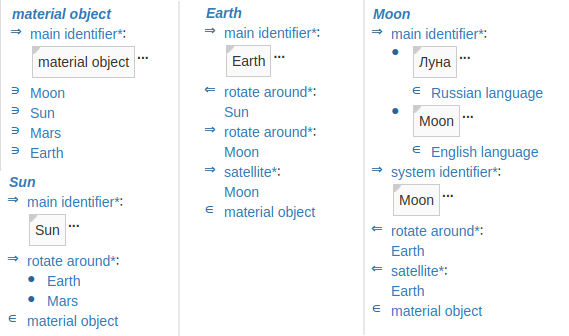
\includegraphics[scale=0.4]{images/intro/scs/example_transf_scn.png}
	\label{scs_example_scn}
\end{figure}

\subsection{Язык представления исходных текстов баз знаний на основе языка LaTeX}
\label{subsec_latex}

Одним из удобных вариантов представления исходных текстов баз знаний для различных областей научно-технической деятельности является Язык представления исходных текстов баз знаний на основе языка LaTeX. В его основу положен язык LaTeX, так как:
\begin{textitemize}
	\item LaTeX это популярный общепринятый язык для записи научно-технических текстов;
	\item LaTeX представляет собой достаточно мощный и легко расширяемый язык;
	\item LaTeX это достаточно строгий и формальный язык, что позволяет реализовать для него транслятор исходных текстов в базу знаний интеллектуальной системы.
\end{textitemize}

Язык представления исходных текстов баз знаний на основе языка LaTeX был разработан для:
\begin{textitemize}
	\item формирования читабельного текста для публикации всего текста \textit{Стандарта OSTIS} или фрагментов в виде печатных изданий;
	\item возможности иметь формальный исходный текст \textit{Стандарта OSTIS}, который может быть протранслирован в базу знаний.
\end{textitemize}

Предлагаемый набор команд условно называется scn-tex (см. \scncite{Ostis-scn-latex-plugin2023}), поскольку в его основу положена идея того, чтобы разработчик писал исходный текст максимально приближенно к тому, как он будет видеть результат компиляции этого исходного текста в SCn-коде и при этом максимально был избавлен от необходимости учитывать особенности языка LaTeX в работе.

Основные принципы разработки исходных текстов баз знаний с использованием scn-tex:
\begin{textitemize}
	\item весь исходный текст стандарта формируется исключительно с использованием набора команд scn-tex;
	\item запрещается использовать любые другие команды для форматирования текста, изменения шрифта, вставки внешних файлов и т.д;
	\item в рамках естественно-языковых фрагментов, входящих в состав стандарта, допускается использование команд LaTeX для вставки специальных символов и математических формул
	\item для добавления файлов изображений в текст стандарта используются только команды scn-tex;
	\item используются для формирования нумерованных и маркированных списков, добавления закрывающих и открывающих скобок различного вида (кроме круглых) используются только команды scn-tex;
	\item для выделения курсивом идентификаторов в рамках естественно-языковых фрагментов, входящих в состав стандарта, используется только команда \textbackslash textit\{\}
	\item для выделения полужирным курсивом используется комбинация команд \textbackslash textbf\{\textbackslash textit\{\}\}
\end{textitemize}

Каждая команда из набора scn-tex начинается с префикса \textbackslash scn, после которого идет имя команды, примерно описывающее то, как связан текущий отображаемый фрагмент текста с описываемой сущностью.

Например:
\begin{textitemize}
	\item \textbackslash scnrelfrom --- дуга ориентированного отношения, которая выходит из описываемой сущности в другую сущность
	\item \textbackslash scnrelto --- дуга ориентированного отношения, которая входит в описываемую сущность
	\item \textbackslash scnnote --- естественно-языковое примечание к описываемой сущности
\end{textitemize}

Полный перечень команд можно увидеть в файле scn.sty (см. \scncite{Ostis-scn-latex-plugin2023}), а примеры использования команд каждого типа --- в исходных текстах стандарта (см. \scncite{Ostis-standart2023}).

Для формирования отступов для корректного отображения sc.n-текстов используется окружение \textbackslash begin\{scnindent\} --- \textbackslash end\{scnindent\}. После смещения на определенное число уровней вправо следует смещение на то же число уровней влево.

Пример исходного текста:

\begin{verbatim}
\scnheader{кибернетическая система}
\scnsuperset{компьютерная система}
\begin{scnindent}
    \scnidtf{искусственная кибернетическая система}
    \scnsuperset{ostis-система}
    \begin{scnindent}
        \scnidtf{компьютерная система, построенная по технологии OSTIS на основе
		 интерпретации спроектированной логико-семантическая sc-модель этой системы}
    \end{scnindent}
\end{scnindent}
\end{verbatim}

Результат компиляции:

\begin{SCn}
\scnheader{кибернетическая система}
\scnsuperset{компьютерная система}
\begin{scnindent}
    \scnidtf{искусственная кибернетическая система}
    \scnsuperset{ostis-система}
    \begin{scnindent}
        \scnidtf{компьютерная система, построенная по технологии OSTIS на основе интерпретации спроектированной логико-семантическая sc-модель этой системы}
    \end{scnindent}
\end{scnindent}
\end{SCn}

\bigskip

Команды из набора scn-tex делятся на классы. К чаще всего используемым классам относятся окружения (environments) и списки (lists), которые являются частным случаем окружения. Окружения могут быть вложенными.

\bigskip

Пример исходного текста:

\bigskip

\begin{verbatim}
\scnheader{Логико-семантическая модель Метасистемы IMS.ostis}
\scnrelfrom{примечание}{
	\begin{scnset}
	\scnfilelong{IMS.ostis}
	\scnrelto{сокращение}{\scnfilelong{Метасистема IMS.ostis}}
	\begin{scnindent}
	\scnrelto{сокращение}{\scnfilelong{Intelligent MetaSystem of Open Semantic Technology
	 for Intelligent Systems}}
	\end{scnindent}
	\end{scnset}
	}
\scnidtf{Логико-семантическая модель интеллектуального ostis-портала научно-технических
 знаний по Технологии OSTIS}
\end{verbatim}

\bigskip

Результат компиляции:

\begin{SCn}
\scnheader{Логико-семантическая модель Метасистемы IMS.ostis}
\scnrelfrom{примечание}{
	\begin{scnset}
	\scnfilelong{IMS.ostis}
	\scnrelto{сокращение}{\scnfilelong{Метасистема IMS.ostis}}
	\begin{scnindent}
	\scnrelto{сокращение}{\scnfilelong{Intelligent MetaSystem of Open Semantic Technology for Intelligent Systems}}
	\end{scnindent}
	\end{scnset}
	}
\scnidtf{Логико-семантическая модель интеллектуального ostis-портала научно-технических знаний по Технологии OSTIS}
\end{SCn}

\bigskip

Таким образом scn-tex позволяет записать практически любую синтаксически корректную конструкцию SCn-кода.

Для трансляции исходного текста в базу знаний был разработан tex2scs-translator (см. \scncite{Ostis-tex2scs-translator2023}), который переводит фрагменты scn-tex в SCs-код. Каждой scn-tex команде соответствует определенная синтаксическая конструкция SCs-кода. Таким образом, весь исходный текст Стандарта OSTIS, записанный в scn-tex, может быть протранслирован в базу знаний любой ostis-системы, которая поддерживает сборку базы знаний из sc.s-файлов. Далее рассмотрим пример работы транслятора.

Текст для трансляции в формате scn-tex:

\begin{verbatim}
	\scnheader{множество}
	\begin{scnrelfromset}{разбиение}
		\scnitem{конечное множество}
		\scnitem{бесконечное множество}
	\end{scnrelfromset}
\end{verbatim}

\bigskip

Результат трансляции в SCs-код:

\begin{verbatim}
	.system_element_0
=> nrel_subdividing: {
	.system_element_1;
	.system_element_2
};;

.system_element_1 => nrel_main_idtf: [конечное множество] (* <- lang_ru;;
 => nrel_format: format_html;; *);;
.system_element_1 <- sc_node;;

nrel_subdividing => nrel_main_idtf: [разбиение*] (* <- lang_ru;; =>
nrel_format: format_html;; *);;
nrel_subdividing <- sc_node_norole_relation;;

.system_element_2 => nrel_main_idtf: [бесконечное множество] (* <- lang_ru;;
 => nrel_format: format_html;; *);;
.system_element_2 <- sc_node;;

.system_element_0 => nrel_main_idtf: [множество] (* <- lang_ru;; => nrel_format:
 format_html;; *);;
.system_element_0 <- sc_node;;

	\end{verbatim}

\section*{Заключение к Главе \ref{chapter_ext_lang}}
В главе были рассмотрены правила идентификации \textit{sc-элементов}, а также \textit{SCg-код}, \textit{SCs-код}, \textit{SCn-код} --- универсальные \textit{внешние языки ostis-систем}, близкие \textit{языку внутреннего смыслового представления знаний}.
\textbf{\textit{SCg-код}} представляет собой способ визуализации \textit{sc-текстов} (\textit{информационных конструкций SC-кода}) в виде рисунков этих абстрактных конструкций.
\textbf{\textit{SCs-код}} представляет собой множество линейных текстов (\textit{sc.s-текстов}), каждый из которых состоит из предложений (\textit{sc.s-предложений}), разделенных друг от друга двойной \textit{точкой с запятой} (разделителем \textit{sc.s-предложений}).
\textbf{\textit{SCn-код}} является языком структурированного внешнего представления текстов \textit{SC-кода} и представляет собой синтаксическое расширение \textit{SCs-кода}, направленное на повышение наглядности и компактности текстов \textit{SCs-кода}.
Для каждого из указанных \textit{внешних языков} были определены \textit{синтаксис} и \textit{денотационная семантика}, приведены примеры описанных с помощью этих \textit{языков} \textit{информационных конструкций}.
%%%%%%%%%%%%%%%%%%%%%%%%% referenc.tex %%%%%%%%%%%%%%%%%%%%%%%%%%%%%%
% sample references
% %
% Use this file as a template for your own input.
%
%%%%%%%%%%%%%%%%%%%%%%%% Springer-Verlag %%%%%%%%%%%%%%%%%%%%%%%%%%
%
% BibTeX users please use
% \bibliographystyle{}
% \bibliography{}
%
\biblstarthook{In view of the parallel print and (chapter-wise) online publication of your book at \url{www.springerlink.com} it has been decided that -- as a genreral rule --  references should be sorted chapter-wise and placed at the end of the individual chapters. However, upon agreement with your contact at Springer you may list your references in a single seperate chapter at the end of your book. Deactivate the class option \texttt{sectrefs} and the \texttt{thebibliography} environment will be put out as a chapter of its own.\\\indent
References may be \textit{cited} in the text either by number (preferred) or by author/year.\footnote{Make sure that all references from the list are cited in the text. Those not cited should be moved to a separate \textit{Further Reading} section or chapter.} If the citatiion in the text is numbered, the reference list should be arranged in ascending order. If the citation in the text is author/year, the reference list should be \textit{sorted} alphabetically and if there are several works by the same author, the following order should be used:
\begin{enumerate}
\item all works by the author alone, ordered chronologically by year of publication
\item all works by the author with a coauthor, ordered alphabetically by coauthor
\item all works by the author with several coauthors, ordered chronologically by year of publication.
\end{enumerate}
The \textit{styling} of references\footnote{Always use the standard abbreviation of a journal's name according to the ISSN \textit{List of Title Word Abbreviations}, see \url{http://www.issn.org/en/node/344}} depends on the subject of your book:
\begin{itemize}
\item The \textit{two} recommended styles for references in books on \textit{mathematical, physical, statistical and computer sciences} are depicted in ~\cite{science-contrib, science-online, science-mono, science-journal, science-DOI} and ~\cite{phys-online, phys-mono, phys-journal, phys-DOI, phys-contrib}.
\item Examples of the most commonly used reference style in books on \textit{Psychology, Social Sciences} are~\cite{psysoc-mono, psysoc-online,psysoc-journal, psysoc-contrib, psysoc-DOI}.
\item Examples for references in books on \textit{Humanities, Linguistics, Philosophy} are~\cite{humlinphil-journal, humlinphil-contrib, humlinphil-mono, humlinphil-online, humlinphil-DOI}.
\item Examples of the basic Springer style used in publications on a wide range of subjects such as \textit{Computer Science, Economics, Engineering, Geosciences, Life Sciences, Medicine, Biomedicine} are ~\cite{basic-contrib, basic-online, basic-journal, basic-DOI, basic-mono}. 
\end{itemize}
}

\begin{thebibliography}{99.}%
% and use \bibitem to create references.
%
% Use the following syntax and markup for your references if 
% the subject of your book is from the field 
% "Mathematics, Physics, Statistics, Computer Science"
%
% Contribution 
\bibitem{science-contrib} Broy, M.: Software engineering --- from auxiliary to key technologies. In: Broy, M., Dener, E. (eds.) Software Pioneers, pp. 10-13. Springer, Heidelberg (2002)
%
% Online Document
\bibitem{science-online} Dod, J.: Effective substances. In: The Dictionary of Substances and Their Effects. Royal Society of Chemistry (1999) Available via DIALOG. \\
\url{http://www.rsc.org/dose/title of subordinate document. Cited 15 Jan 1999}
%
% Monograph
\bibitem{science-mono} Geddes, K.O., Czapor, S.R., Labahn, G.: Algorithms for Computer Algebra. Kluwer, Boston (1992) 
%
% Journal article
\bibitem{science-journal} Hamburger, C.: Quasimonotonicity, regularity and duality for nonlinear systems of partial differential equations. Ann. Mat. Pura. Appl. \textbf{169}, 321--354 (1995)
%
% Journal article by DOI
\bibitem{science-DOI} Slifka, M.K., Whitton, J.L.: Clinical implications of dysregulated cytokine production. J. Mol. Med. (2000) doi: 10.1007/s001090000086 
%
\bigskip

% Use the following (APS) syntax and markup for your references if 
% the subject of your book is from the field 
% "Mathematics, Physics, Statistics, Computer Science"
%
% Online Document
\bibitem{phys-online} J. Dod, in \textit{The Dictionary of Substances and Their Effects}, Royal Society of Chemistry. (Available via DIALOG, 1999), 
\url{http://www.rsc.org/dose/title of subordinate document. Cited 15 Jan 1999}
%
% Monograph
\bibitem{phys-mono} H. Ibach, H. L\"uth, \textit{Solid-State Physics}, 2nd edn. (Springer, New York, 1996), pp. 45-56 
%
% Journal article
\bibitem{phys-journal} S. Preuss, A. Demchuk Jr., M. Stuke, Appl. Phys. A \textbf{61}
%
% Journal article by DOI
\bibitem{phys-DOI} M.K. Slifka, J.L. Whitton, J. Mol. Med., doi: 10.1007/s001090000086
%
% Contribution 
\bibitem{phys-contrib} S.E. Smith, in \textit{Neuromuscular Junction}, ed. by E. Zaimis. Handbook of Experimental Pharmacology, vol 42 (Springer, Heidelberg, 1976), p. 593
%
\bigskip
%
% Use the following syntax and markup for your references if 
% the subject of your book is from the field 
% "Psychology, Social Sciences"
%
%
% Monograph
\bibitem{psysoc-mono} Calfee, R.~C., \& Valencia, R.~R. (1991). \textit{APA guide to preparing manuscripts for journal publication.} Washington, DC: American Psychological Association.
%
% Online Document
\bibitem{psysoc-online} Dod, J. (1999). Effective substances. In: The dictionary of substances and their effects. Royal Society of Chemistry. Available via DIALOG. \\
\url{http://www.rsc.org/dose/Effective substances.} Cited 15 Jan 1999.
%
% Journal article
\bibitem{psysoc-journal} Harris, M., Karper, E., Stacks, G., Hoffman, D., DeNiro, R., Cruz, P., et al. (2001). Writing labs and the Hollywood connection. \textit{J Film} Writing, 44(3), 213--245.
%
% Contribution 
\bibitem{psysoc-contrib} O'Neil, J.~M., \& Egan, J. (1992). Men's and women's gender role journeys: Metaphor for healing, transition, and transformation. In B.~R. Wainrig (Ed.), \textit{Gender issues across the life cycle} (pp. 107--123). New York: Springer.
%
% Journal article by DOI
\bibitem{psysoc-DOI}Kreger, M., Brindis, C.D., Manuel, D.M., Sassoubre, L. (2007). Lessons learned in systems change initiatives: benchmarks and indicators. \textit{American Journal of Community Psychology}, doi: 10.1007/s10464-007-9108-14.
%
%
% Use the following syntax and markup for your references if 
% the subject of your book is from the field 
% "Humanities, Linguistics, Philosophy"
%
\bigskip
%
% Journal article
\bibitem{humlinphil-journal} Alber John, Daniel C. O'Connell, and Sabine Kowal. 2002. Personal perspective in TV interviews. \textit{Pragmatics} 12:257--271
%
% Contribution 
\bibitem{humlinphil-contrib} Cameron, Deborah. 1997. Theoretical debates in feminist linguistics: Questions of sex and gender. In \textit{Gender and discourse}, ed. Ruth Wodak, 99--119. London: Sage Publications.
%
% Monograph
\bibitem{humlinphil-mono} Cameron, Deborah. 1985. \textit{Feminism and linguistic theory.} New York: St. Martin's Press.
%
% Online Document
\bibitem{humlinphil-online} Dod, Jake. 1999. Effective substances. In: The dictionary of substances and their effects. Royal Society of Chemistry. Available via DIALOG. \\
http://www.rsc.org/dose/title of subordinate document. Cited 15 Jan 1999
%
% Journal article by DOI
\bibitem{humlinphil-DOI} Suleiman, Camelia, Daniel C. O'Connell, and Sabine Kowal. 2002. `If you and I, if we, in this later day, lose that sacred fire...': Perspective in political interviews. \textit{Journal of Psycholinguistic Research}. doi: 10.1023/A:1015592129296.
%
%
%
\bigskip
%
%
% Use the following syntax and markup for your references if 
% the subject of your book is from the field 
% "Computer Science, Economics, Engineering, Geosciences, Life Sciences"
%
%
% Contribution 
\bibitem{basic-contrib} Brown B, Aaron M (2001) The politics of nature. In: Smith J (ed) The rise of modern genomics, 3rd edn. Wiley, New York 
%
% Online Document
\bibitem{basic-online} Dod J (1999) Effective Substances. In: The dictionary of substances and their effects. Royal Society of Chemistry. Available via DIALOG. \\
\url{http://www.rsc.org/dose/title of subordinate document. Cited 15 Jan 1999}
%
% Journal article by DOI
\bibitem{basic-DOI} Slifka MK, Whitton JL (2000) Clinical implications of dysregulated cytokine production. J Mol Med, doi: 10.1007/s001090000086
%
% Journal article
\bibitem{basic-journal} Smith J, Jones M Jr, Houghton L et al (1999) Future of health insurance. N Engl J Med 965:325--329
%
% Monograph
\bibitem{basic-mono} South J, Blass B (2001) The future of modern genomics. Blackwell, London 
%
\end{thebibliography}
